\documentclass{article}

\usepackage[utf8]{inputenc}

\usepackage{amsmath, bm}
\usepackage{graphicx}
\usepackage{amssymb}
\usepackage{float}
\usepackage{caption}
\usepackage{subcaption}
\usepackage{hyperref}
% set font size to 11pt
% set margin
\usepackage[margin=0.5in]{geometry}

\setlength{\parskip}{\baselineskip}%
\setlength{\parindent}{0pt}%

\begin{document}

% insert pdf cover page here

\title{Full Technical Report: 3A3 Supersonic Nozzle}
\author{lwp26}
\date{December 2023}
\maketitle

\begin{abstract}
    \centering
    % write a brief summary of the experiment and the results
    Theory of 1D compressible flow for convergent divergent nozzles was discussed and compared to experimental results.
    The static pressure distribution along the nozzle was measured for four different flow cases, for which the locations of choking points and a normal shock were found.
    Theory of mass flow rate through an orifice plate and use of a discharge coefficient were discussed and used to calculate the mass flow rates, throat areas and exit areas.
    Extensive uncertainty analysis was conducted and discussed for all measurements and calculated results.
    Optical theory of Schlieren and shadowgraph visualisation techniques were discussed and used to visualise the normal shock wave in the supersonic wind tunnel.
    Measurements of stagnation and static pressure of the free stream in a Mach 1.5 wind tunnel were taken during startup and working state which were explained by compressible flow theory.
\end{abstract}

\newpage

\section{Introduction}

\subsection{Purpose}
% explaining the significance of supersonic nozzles to wind tunnels and other applications.
% The converging-diverging nozzle is a device that can accelerate a fluid to supersonic speeds, and is used in both aircraft and wind tunnels.
In the design of bluff or streamlined supersonic bodies, it is essential to understand the aerodynamic forces and flow patterns that occur at high speeds.
This can be done in a frame of reference of the lab by using wind tunnels.
Operating costs of high flow rate tunnels are immense, and so dimensional analysis is used for the testing of smaller models in a smaller tunnel.
Convergent-divergent nozzles are a fundamental component of wind tunnels, and so it is important to understand their influence on flow over a range of operating points.
They are also used to achieve efficient turbomachinery, rocket propulsion and industrial processes involving high speed flow.
% explain the purpose of the experiment

\subsection{Objectives}
% list the objectives of the experiment

\subsubsection{Part 1}

\begin{itemize}
    \item To study the development of flow in a converging-diverging nozzle for 4 different pressure ratios across the nozzle.
    \item To observe phenomena of choking and compare results to adiabatic, inviscid theory.
    \item To appreciate the validity and limitations of one-dimensional, adiabatic, inviscid theory.
\end{itemize}

\subsubsection{Part 2}

\begin{itemize}
    \item To become familiar with features of a supersonic wind tunnel and visualisation techniques.
    \item To observe changes flow behaviour due to the formation of a normal shock wave.
\end{itemize}

\section{Theory}
% Introduce the essential relationships necessary to explain your results in the later section. Refer to these
% equations in the later sections. (You need not derive these relationships but you should explain in words why
% they are needed and reference their source).

\subsection{Mass flow rate though orifice plate}

The following assumptions are made to derive a relationship for the mass flow rate through an orifice plate.
\begin{itemize}
    \item The flow into the orifice is inviscid,
    \item The flow is slow enough to be treated as incompressible with density equal to that in the atmosphere upstream of the orifice (where the velocity is negligible),
    \item The velocity is uniform across the plane of the orifice,
    \item The pressure difference between the orifice plane and the upstream atmosphere is that measured on the water manometer
\end{itemize} 

With both the inviscid and incompressible assumptions, the ideal flow rate through the orifice can be calculated using the pressure difference between the orifice plane and the upstream atmosphere is that measured on the
water manometer. By applying the Bernoulli equation from the upstream atmosphere (1) to the orifice plane (2),

\begin{equation}
    p_1 = p_2 + \frac{1}{2} \rho_a v_2^2
\end{equation}

Where $A$ and $v_2$ are the cross-sectional area, and velocity at the orifice. The pressure in the centre of the orifice is taken to be equal to the value measured at the wall, due to the assumption that the velocity is uniform across the orifice plane.
The theoretical mass flow rate through the orifice is then given by the following equation.
\begin{equation}
    \dot{m}_\text{ideal} = \rho_a A v_2 = \rho_a \left( \frac{\pi D^2}{4}\right) \sqrt{\frac{2(p_1-p_2)}{\rho_a}} \;\;\;\;\;\; \text{where} \;\;\;\;\;\ p_2 - p_1 = \rho_w g \Delta h
\end{equation}
Where $\rho_a$ is the density of air and $\rho_w$ is the density of water used for the manometer.

However, the actual flow rate through the orifice differs from the theoretical value as our assumptions are not valid.
The first assumption is not valid as there is significant viscous dissipation before the orifice.
However, these losses are accounted for by a discharge coefficient $C_d$, which is defined as the ratio of actual discharge to the ideal discharge.
The value of $C_d$ is constant at the high Reynolds numbers considered in this report.
To analyse the validity of the second assumption, consider the case of maximum flow, when the nozzle is choked upstream of the orifice, then its non-dimensional mass flow rate is given by the following equation.
\begin{equation}
    \frac{\dot{m}\sqrt{c_pT_0}}{p_0A^*} = 1.281
\end{equation}
From this, the non-dimensional mass flow rate at the orifice can be calculated using the area ratio of the orifice to the nozzle throat.
The area of the throat is approximately $24\text{mm}^2$, and so the non-dimensional mass flow rate at the orifice is $0.1282$.
At this point, the corresponding density ratio $\rho/\rho_0 = 0.9997 \approx 1$. This means that the density change is negligible and can be ignored.

The third assumption that the velocity is uniform is also poor, and is accounted for by the discharge coefficient $C_d$.
This difference is characterised by the discharge coefficient $C_d$ which is defined as the ratio of the actual flow rate to the theoretical flow rate.
\begin{equation}
    \dot{m}_\text{actual} = C_d \dot{m}_\text{ideal}
\end{equation}

The discharge coefficient of the orifice is effectively constant over the range of high Reynolds numbers considered in this experiment.
This was shown by Graham and Webster \cite{Graham_K_Webster:2019} in figure \ref{fig:const_Cd_Re}.

\subsection{Pressure tappings}
The assumption that flow is uniform is used here such that the pressure at the wall is equal to the pressure at the centre of the nozzle.
The static pressure at a specific pressure tapping along the nozzle is given by the following equation.
\begin{equation}
    p = p_0 - \rho_{Hg} g \Delta h
\end{equation}
Where $\rho_{Hg}$ is the density of mercury and $\Delta h$ is the height difference of mercury between the specific pressure tapping and atmospheric tapping.

The static pressure ratio across the nozzle is given by the following equation.
\begin{equation}
    \frac{p}{p_0} = 1 - \frac{\rho_{Hg} g \Delta h}{p_0}
\end{equation}

\subsection{Compressible flow theory}
Theory of 1D compressible flow can be used to predict flow behaviour in converging and diverging nozzles.
The flow can be assumed to be adiabatic, and isentropic in cases 1, 2 and 4.
It can also be taken to be isentropic up to the shock wave in case 3.
The following equation can be derived from considering the differential forms of continuity and ideal gas relations.
\begin{equation}
    (M^2 - 1)\frac{dV}{V} = \frac{dA}{A}
    \label{eqn:condiv_theory}
\end{equation}
This shows for a converging nozzle where $dA < 0$, the flow is either subsonic and accelerating, or supersonic and decelerating.
For a diverging nozzle, $dA > 0$, the flow is either subsonic and decelerating, or supersonic and accelerating.

For a given static pressure ratio across the nozzle, the Mach number can be found by rearanging the following equation.
\begin{equation}
    \frac{p}{p_0} = \left( 1 + \frac{\gamma - 1}{2}M^2\right) ^ {-\frac{\gamma}{\gamma-1}} \implies M = \sqrt{\frac{2}{\gamma-1} \left( \left( \frac{p}{p_0}\right) ^ {-\frac{\gamma-1}{\gamma}} - 1\right)}
\end{equation}

For case 3 there is thought to be a normal shock wave and so the flow is not isentropic, however the location can be estimated, and drop in stagnation pressure across the shock wave can be accounted for.
This is done by dividing the original static pressure ratio by the ratio of stagnation pressures across the shock wave.
\begin{equation}
    \frac{p}{p_{0s}} = \frac{p/p_0}{p_{0s}/p_0}
\end{equation}
The stagnant pressure before and after the shock is given by $p_0$ and $p_{0s}$ respectively.
The stagnation pressure ratio across the shock wave is given in the databook \cite{data_book}.
\begin{equation}
    \frac{p_{0s}}{p_0} = \left( \frac{\frac{\gamma+1}{2}M^2}{1 + \frac{\gamma-1}{2}M^2}\right) ^ \frac{\gamma}{\gamma-1} \left( \frac{2\gamma}{\gamma+1} M^2 - \frac{\gamma-1}{\gamma+1}\right) ^ \frac{1}{1 - \gamma}
\end{equation}
Where $M$ is the Mach number before the shock wave.
The nozzle area ratio can also be found using the following equation from the Mach number.
\begin{equation}
    \frac{A}{A^*} = \frac{1}{M} \left( \frac{2}{\gamma+1} \left( 1 + \frac{\gamma-1}{2}M^2\right) \right) ^ {\frac{\gamma+1}{2(\gamma-1)}}
\end{equation}
However, using the value of $\dot{m}$ calculated from the pressure drop across the Orifice plate, the exact area at any point can be found using the dimensionless mass flow rate given below.
\begin{equation}
    A = \frac{\dot{m}\sqrt{c_pT_0}}{p_0} \left( \frac{\dot{m}\sqrt{c_pT_0}}{p_0A} \right)^{-1}
    \label{eqn:area}
\end{equation}
As $C_p$, $T_0$ and $p_0$ are known, the area can be found from the Mach number.
This is only a function of the Mach number, as seen below
\begin{equation}
    \frac{\dot{m}\sqrt{c_pT_0}}{p_0A} = \frac{\gamma}{\sqrt{\gamma-1}} M \left(1 + \frac{\gamma - 1}{2} M^2 \right) ^ {- \frac{1}{2}\frac{\gamma + 1}{\gamma - 1}} 
\end{equation}

\subsection{Visualisation Techniques}

\subsubsection{Schlieren Visualisation Technique}

The setup for the Schlieren visualisation technique is shown in figure \ref{fig:xz_shlierian}.
The light source is placed at the focal point of the first mirror, such to get collimated light through the tunnel.
The second mirror focuses the light onto a knife edge, where density gradients in the direction normal to the knife edge cause light rays to be deflected, and so some light reaches the camera.
Figure \ref{fig:xz_shlierian} shows rays deflected by horizontal density gradients are blocked by the knife edge.
Figure \ref{fig:yz_shlierian} shows rays deflected by positive density gradients pass, but rays deflected by negative density gradients are blocked.

\begin{figure}[H]
    \centering
    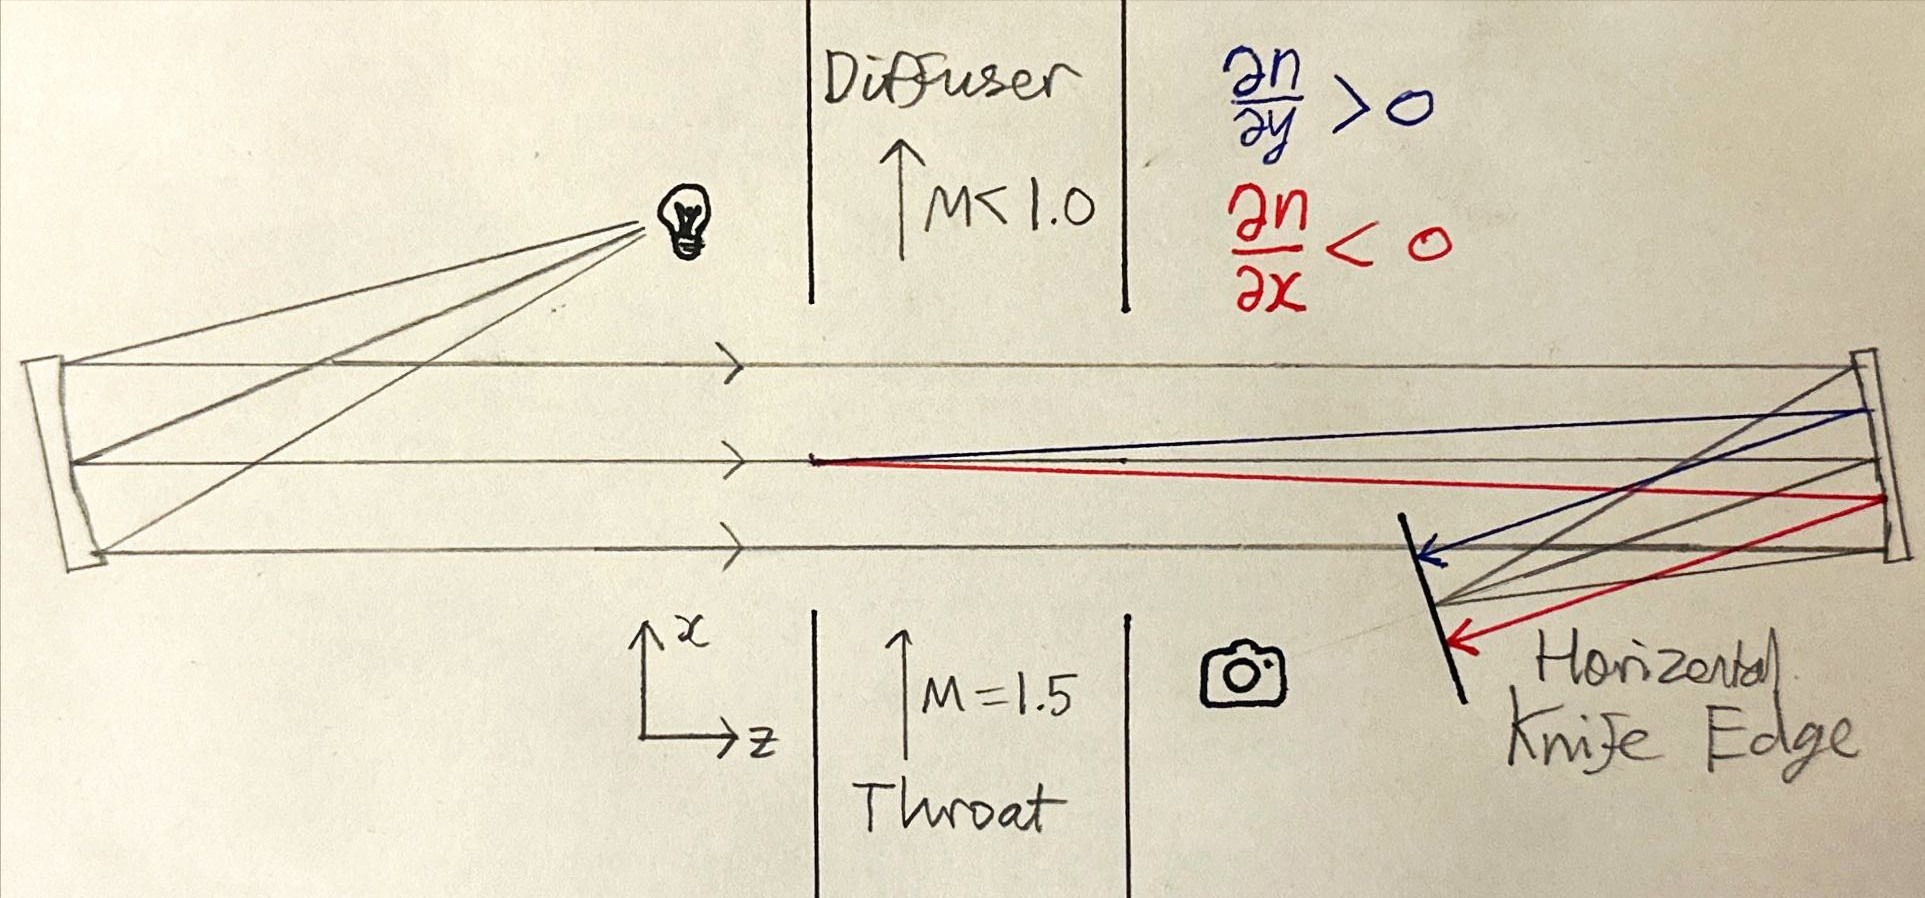
\includegraphics[width=0.8\textwidth]{xz_shlierian.jpg}
    \caption{Sketch of light rays passing through refractive index gradient in XZ plane.}
    \label{fig:xz_shlierian}
\end{figure}

\begin{figure}[H]
    \centering
    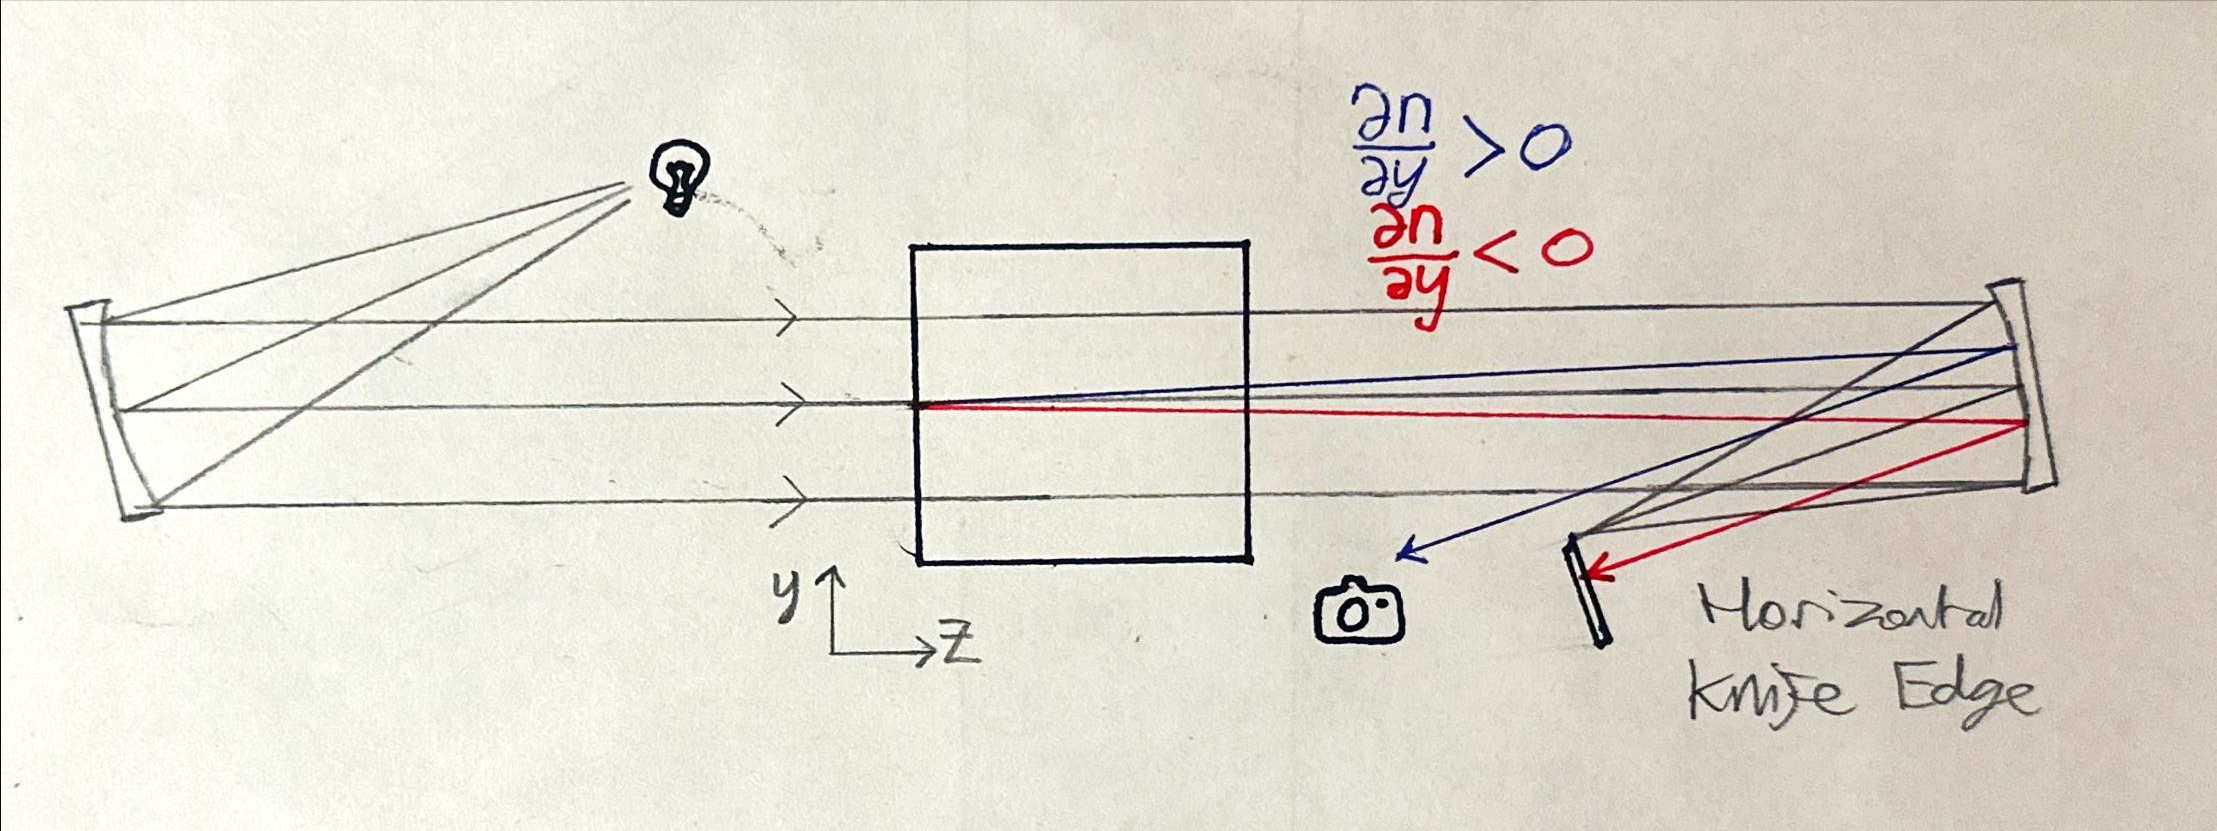
\includegraphics[width=0.8\textwidth]{yz_shlierian.jpg}
    \caption{Sketch of light rays passing through refractive index gradient in YZ plane.}
    \label{fig:yz_shlierian}
\end{figure}

Equations \ref{eqn:refractive_index_gradient} derived by Mazumdar \cite{Mazumdar_Amrita:2013} shown in the appendix, indicate it is not the refractive index, $n$, causing ray deflection, but the gradient $\partial n / \partial y$ of this refractive index.
It is also explained that light ray deflections bend towards regions of higher refractive index.
The relation between the refractive index and density of air is shown to be approximately linear in figure \ref{fig:refractive_index_vs_density} from literature \cite{refractiveindex_info} \cite{Ciddor:96}.

Considering a normal shock wave, the density can be considered as a Heaviside step function of y.
This is because the thickness of the shock is on the order of a few molecular-mean-free paths \cite{babinsky_delery:2011}.
From the linear relation of refractive index and density, the refractive index is also a step function, and so its derivative is a Dirac Delta function.
When integrated over the thickness of the shock, as in equation \ref{eqn:refractive_index_gradient}, this gives an angle of deflection proportional to density gradient.
This means that wider, darker bands with a larger angle of deflection correspond to regions of higher density gradient, and so are stronger shock waves.

For regions of negative density gradient, the light rays are deflected towards the knife edge and so are blocked, and so appear dark in the image.
For regions of positive density gradient, the light rays are deflected away from the knife edge and so pass through, and so appear bright in the image.

A normal shock down the tunnel has a positive density gradient in the $x$ direction, and little density gradient in the $y$ direction.
This means the knife edge should be placed vertically in the image, and the shock wave should appear as a dark band, with a light band in the downstream direction of it.

\subsubsection{Shadowgraph Visualisation Technique}

The setup for the shadowgraph visualisation technique is identical to the Schlieren visualisation technique, except the knife edge is removed.
This means that density gradients in any direction are visible, including those in positive and negative $x$ and $y$ directions.
This means that the only difference is that the shadowgraph produces an image of the second derivative of the density field.

\section{Method}
\subsection{Part 1}
\subsubsection{Apparatus}

\begin{figure}[H]
    \centering
    \begin{subfigure}{0.8\textwidth}
        \centering
        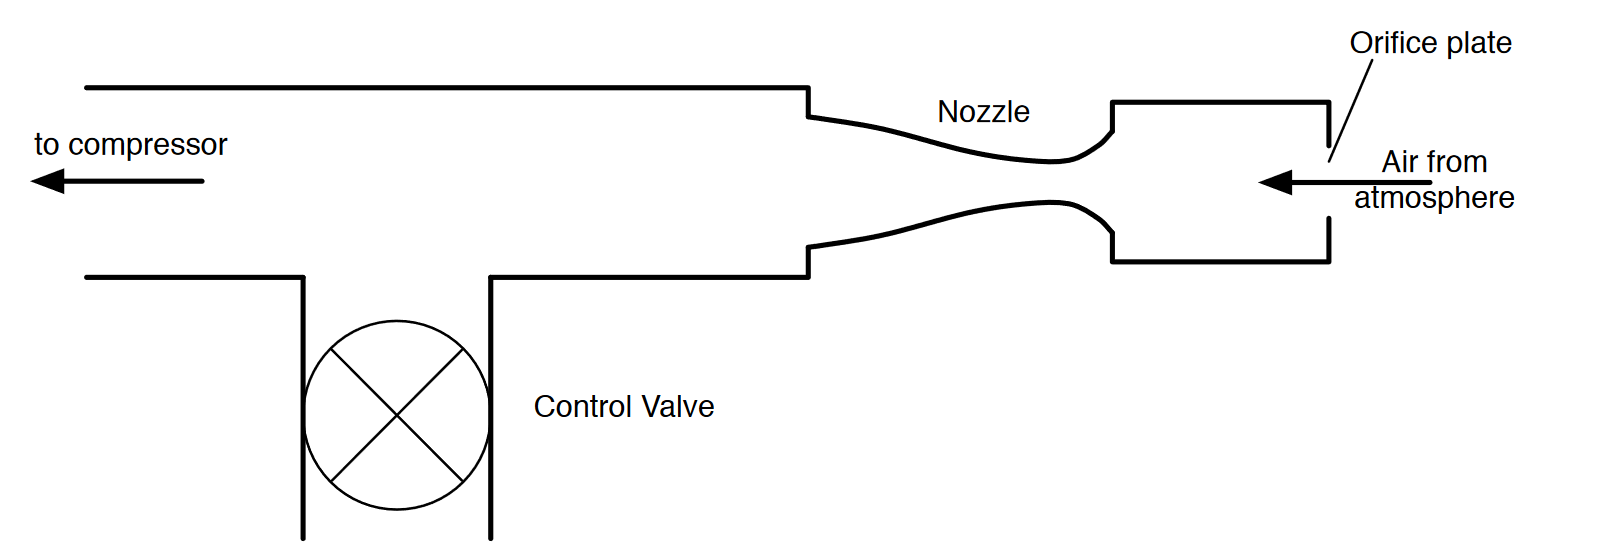
\includegraphics[width=0.6\textwidth]{flow_layout.png}
        \caption{Flow path diagram}
        \label{fig:flow_layout}
    \end{subfigure}
    ~
    \begin{subfigure}{0.8\textwidth}
        \centering
        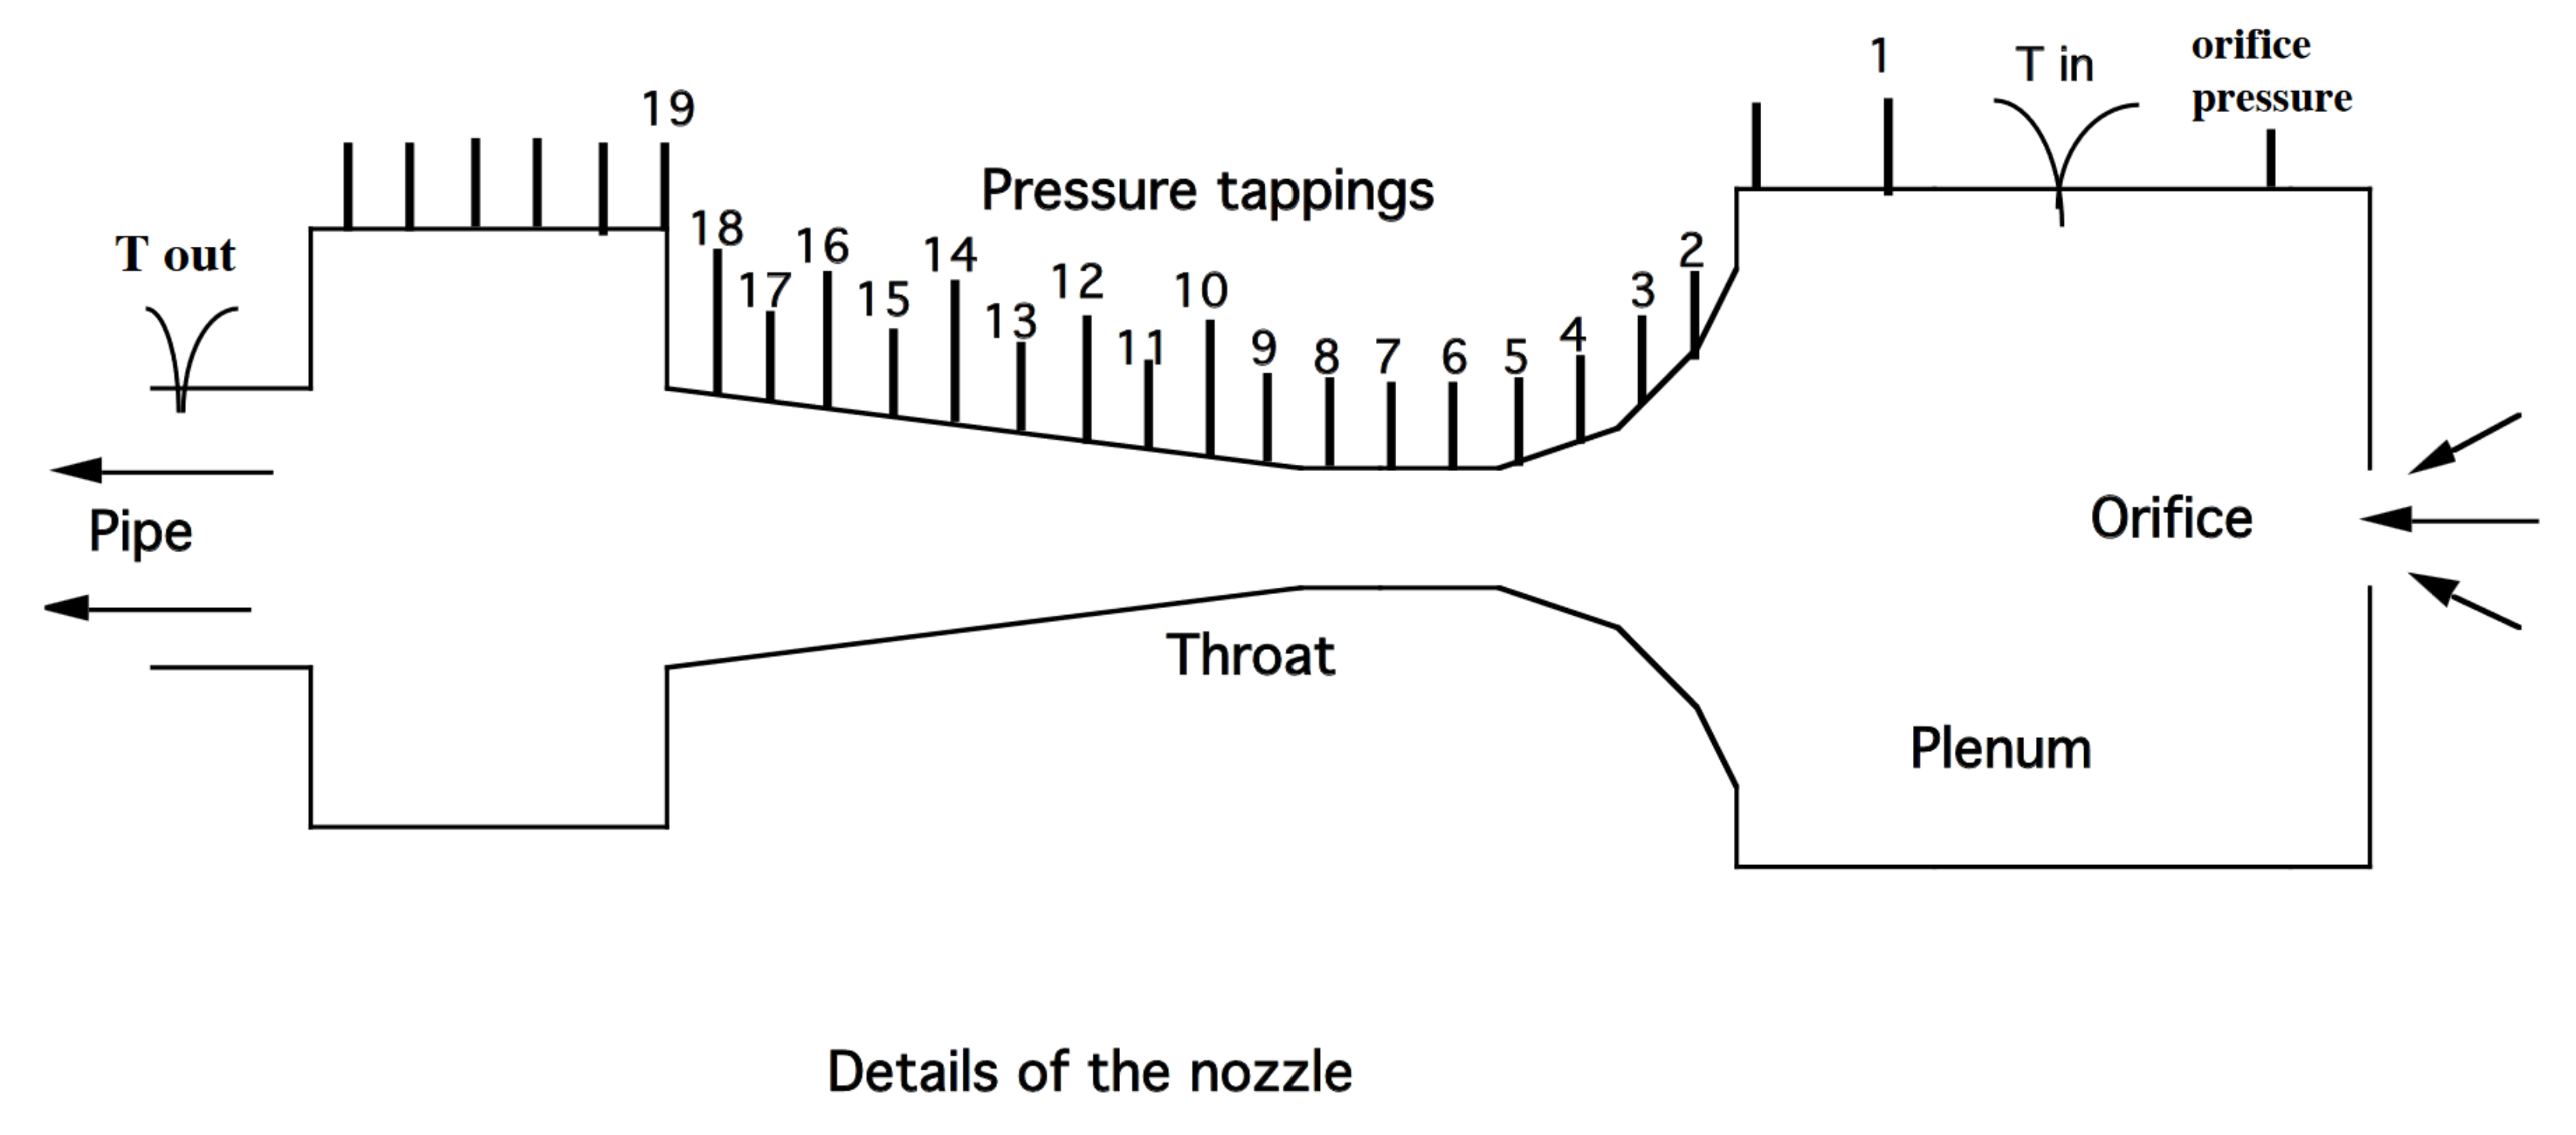
\includegraphics[width=0.6\textwidth]{../Supersonic_Nozzle/small_nozzle_layout.png}
        \caption{Nozzle layout diagram}
        \label{fig:nozzle_layout}
    \end{subfigure}
    \caption{Experiment apparatus \cite{lab_manual}.}
\end{figure}

The apparatus used in this experiment is shown in figure \ref{fig:flow_layout}.
A control valve is used to control the pressure of the air downstream of the nozzle. By closing the valve, the pressure downstream of the nozzle decreases, and so pressure ratio across the nozzle increases.
The pressure at each tapping along the nozzle is measured using a series of 19 vertical mercury manometers.
The pressure difference across the orifice is a smaller pressure drop and so is measured using a vertical water manometer.

\subsubsection{Procedure}

Values for temperature and atmospheric pressure were taken from a gauge and mercury manometer in the lab.
A preliminary experiment was conducted to determine the pressure ratio at which the nozzle is choked.
This was done by closing the valve and increasing the pressure ratio across the nozzle until there was no change in the orifice plate manometer readings.
This approximate height difference of the manometer at the choking point was then recorded.

Then the first operating point was reached by setting the height difference of the manometer to $70\%$ of that of the choking point.
This took a few iterations of adjusting the control valve, waiting for the water manometer to settle and reading both manometers to find the height difference.
After a stable setpoint is reached, the measured orifice manometer height readings were recorded. 
Then all 19 manometer wall tappings and the atmospheric were recorded.
It was noted that tapping 8 had the lowest pressure and so was taken to be the throat of the nozzle.

The second operating point was then reached by setting the height difference of the manometer that of the choking point.
Recording of orifice manometer height readings and all 19 manometer wall tappings and the atmospheric were repeated.

The third operating point is when a shock forms in the diverging part of the nozzle. The valve was closed until the manometer height at the throat, at tapping 8, was equal to the height at tapping 16.
This was because the location of the shock wave was approximated to be where the flow dropped below Mach 1.
This was found to be particularly difficult as the manometer height at tapping 16 was very sensitive to changes in the valve position.
A sufficient setpoint was found and the orifice plate manometer height readings were recorded.
Then again all 19 manometer wall tappings and the atmospheric were recorded.

The fourth and final run was conducted by closing the valve entirely so there was maximum pressure ratio across the nozzle.
Then the orifice plate manometer heights, all 19 manometer wall tappings and the atmospheric were recorded.

\subsection{Uncertainty}

Naturally, there are sources of uncertainty in all measurements taken and so it is important for all calculations to include an estimate of the uncertainty in the final result.
The uncertainty equations are derived from the equation for the quantity being calculated where relative uncertainty of $x$ is given by $u(x)$.
To simplify the analysis the uncertainty in densities of water and mercury are assumed to be negligible.
The uncertainty in pressure ratio is calculated using the following equation.
\begin{equation}
    u\left( \frac{p}{p_0} \right) = u(\Delta h) + u(p_0) = \sqrt{u(h_2)^2+u(h_1)^2} + u(p_0)
\end{equation}
Where $u(h_2)$ and $u(h_1)$ are the relative uncertainties in the height of the manometer calculated from the resolution of the ruler which was 2mm and so the absolute uncertainty is $\pm 1$mm.
The uncertainty in mass flow rate is calculated using the following equation.
\begin{equation}
    u(\dot{m}) = u(C_d) + 2u(D) + \frac{1}{2}u(\rho_a) + \frac{1}{2}u(\Delta H)
\end{equation}
Where $\Delta H$ is the height difference of the water oriface plate manometer, $D$ is the diameter of the oriface plate and $C_d$ is the discharge coefficient.
The uncertainty in manometer height difference is calculated identically to that in the pressure ratio equation.
The absolute uncertainty of diameter and discharge coefficient is taken to be at the resolution given which is $\pm 0.01$mm and $\pm 0.005$ respectively.
% dM2 = - 2 / g * rp ** (-((g-1)/g) - 1)
The uncertainty in Mach number is calculated using the following equation.
\begin{equation}
    u(M) = u\left( \frac{p}{p_0} \right) \frac{d M ( p/p_0 ) }{d (p/p_0)} = u\left(\frac{p}{p_0}\right) \times \frac{2}{\gamma}  \left( \frac{p}{p_0} \right) ^ {\frac{1}{\gamma}}
\end{equation}
The uncertainty for area calculated from dimensionless mass flow rate in equation \ref{eqn:area} is calculated using the following equation.
\begin{equation}
    u(A) = u(\dot{m}) + u\left(\frac{\dot{m}\sqrt{c_pT_0}}{p_0A}\right) + u(T_0) + u(p_0)
\end{equation}
Further uncertainty analysis in dimensionless mass flow rate, area ratio and stagnant pressure ratio across the shock wave is covered in the appendix.
Uncertainty analysis is not conducted for the location of the shock wave as this is already a very rough approximation due to boundary layer effects.

\subsection{Part 2}

\subsubsection{Apparatus}

Layout of Cambridge University Engineering Department's supersonic wind tunnel is shown in figure \ref{fig:supersonic_tunnel}.

\begin{figure}[H]
    \centering
    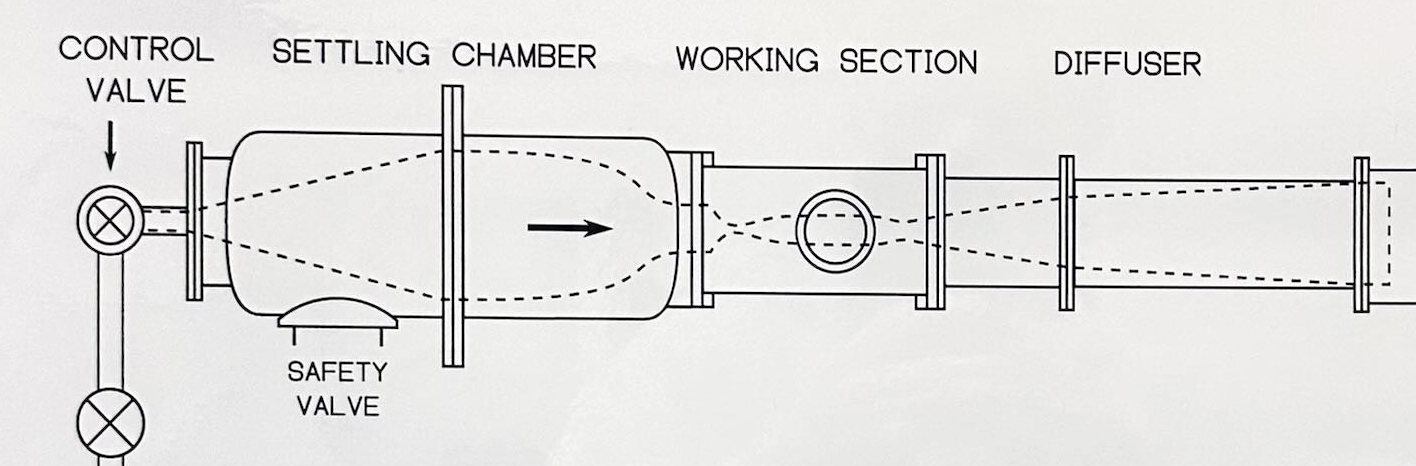
\includegraphics[width=0.8\textwidth]{supersonic_layout.png}
    \caption{Supersonic wind tunnel layout}
    \label{fig:supersonic_tunnel}
\end{figure}

Air is supplied from gas tanks in the basement of the building, and so tests can only be conducted for a limited time, and the valve must be manually adjusted to maintain a constant pressure ratio across the nozzle.
Digital pressure sensors were used to measure the static and stagnation pressure at the same point along the working section.
An additional sensor was used far upstream in the settling chamber to measure the stagnation pressure of the incoming flow.

\subsubsection{Procedure}

Recording of the pressure sensors was started and then the control valve was manually opened.
Shadowgraph images were taken of the normal shockwave on startup and working state of the tunnel.
The tunnel was then turned off and after pressure returned to atmospheric, recording was stopped.

\section{Results}

\begin{center}
    \begin{tabular}{|c|c|c|c|c|c|}
    \hline 
    Case & Throat Mach No.  & Exit Mach No. & Mass flow rate & Throat Area & Exit Area\\
     & (-) & (-) & $\times 10^{-3}$ kg/s & $mm^2$ & $mm^2$ \\
    \hline 
    1 & $0.602\pm 0.003$ & $0.491\pm 0.005$ & $ 4.25\pm 0.42  $ & $21.86 \pm 2.48 $ & $25.02 \pm 2.85 $ \\
    2 & $1.063\pm 0.017$ & $0.715\pm 0.007$ & $ 4.96\pm 0.36  $ & $21.57 \pm 1.80 $ & $23.30 \pm 2.01 $ \\
    3 & $1.063\pm 0.017$ & $0.800\pm 0.036$ & $ 4.96\pm 0.36 $ & $21.57 \pm 1.80 $ & $22.32 \pm 2.21 $ \\
    4 & $1.068\pm 0.017$ & $1.420\pm 0.064$ & $ 4.96\pm 0.36 $ & $21.58 \pm 1.81 $ & $24.21 \pm 2.87 $ \\
    \hline
    \end{tabular}
    \captionsetup{hypcap=true}
    \captionof{table}{Mass flow rates, Mach numbers and nozzle areas for throat and exit for each case.}
    \label{tab:1}
\end{center}
 
\begin{figure}[H]
    \centering
    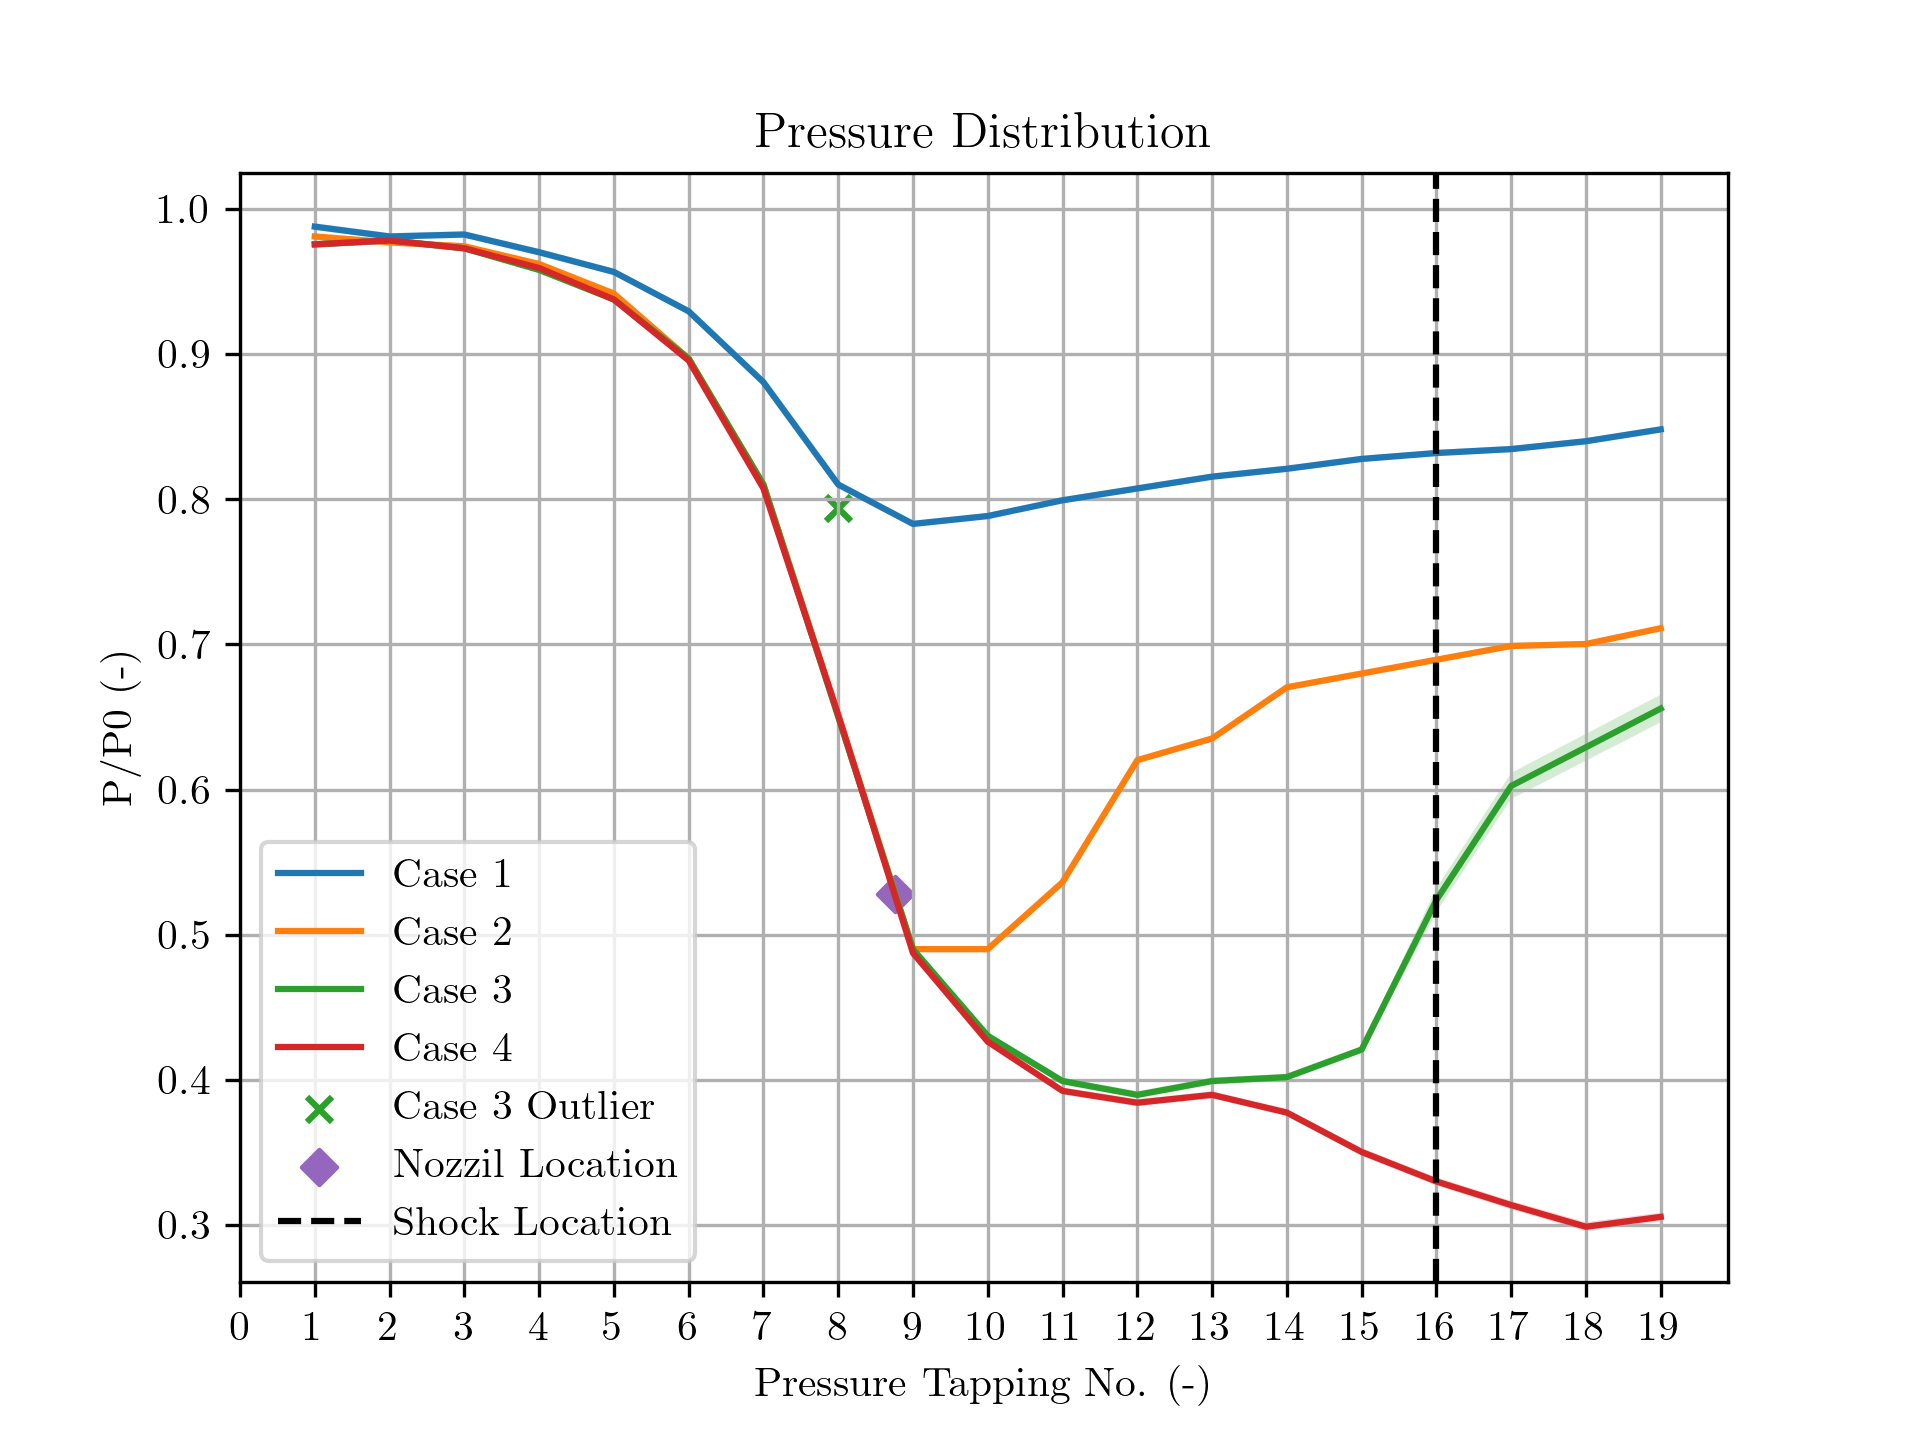
\includegraphics[width=0.98\textwidth]{../Supersonic_Nozzle/pressure_ratio_distribution_corrected.png}
    \caption{Static pressure ratio distribution along the nozzle.}
    \label{fig:pressure_distribution}
\end{figure}

\begin{figure}[H]
    \centering
    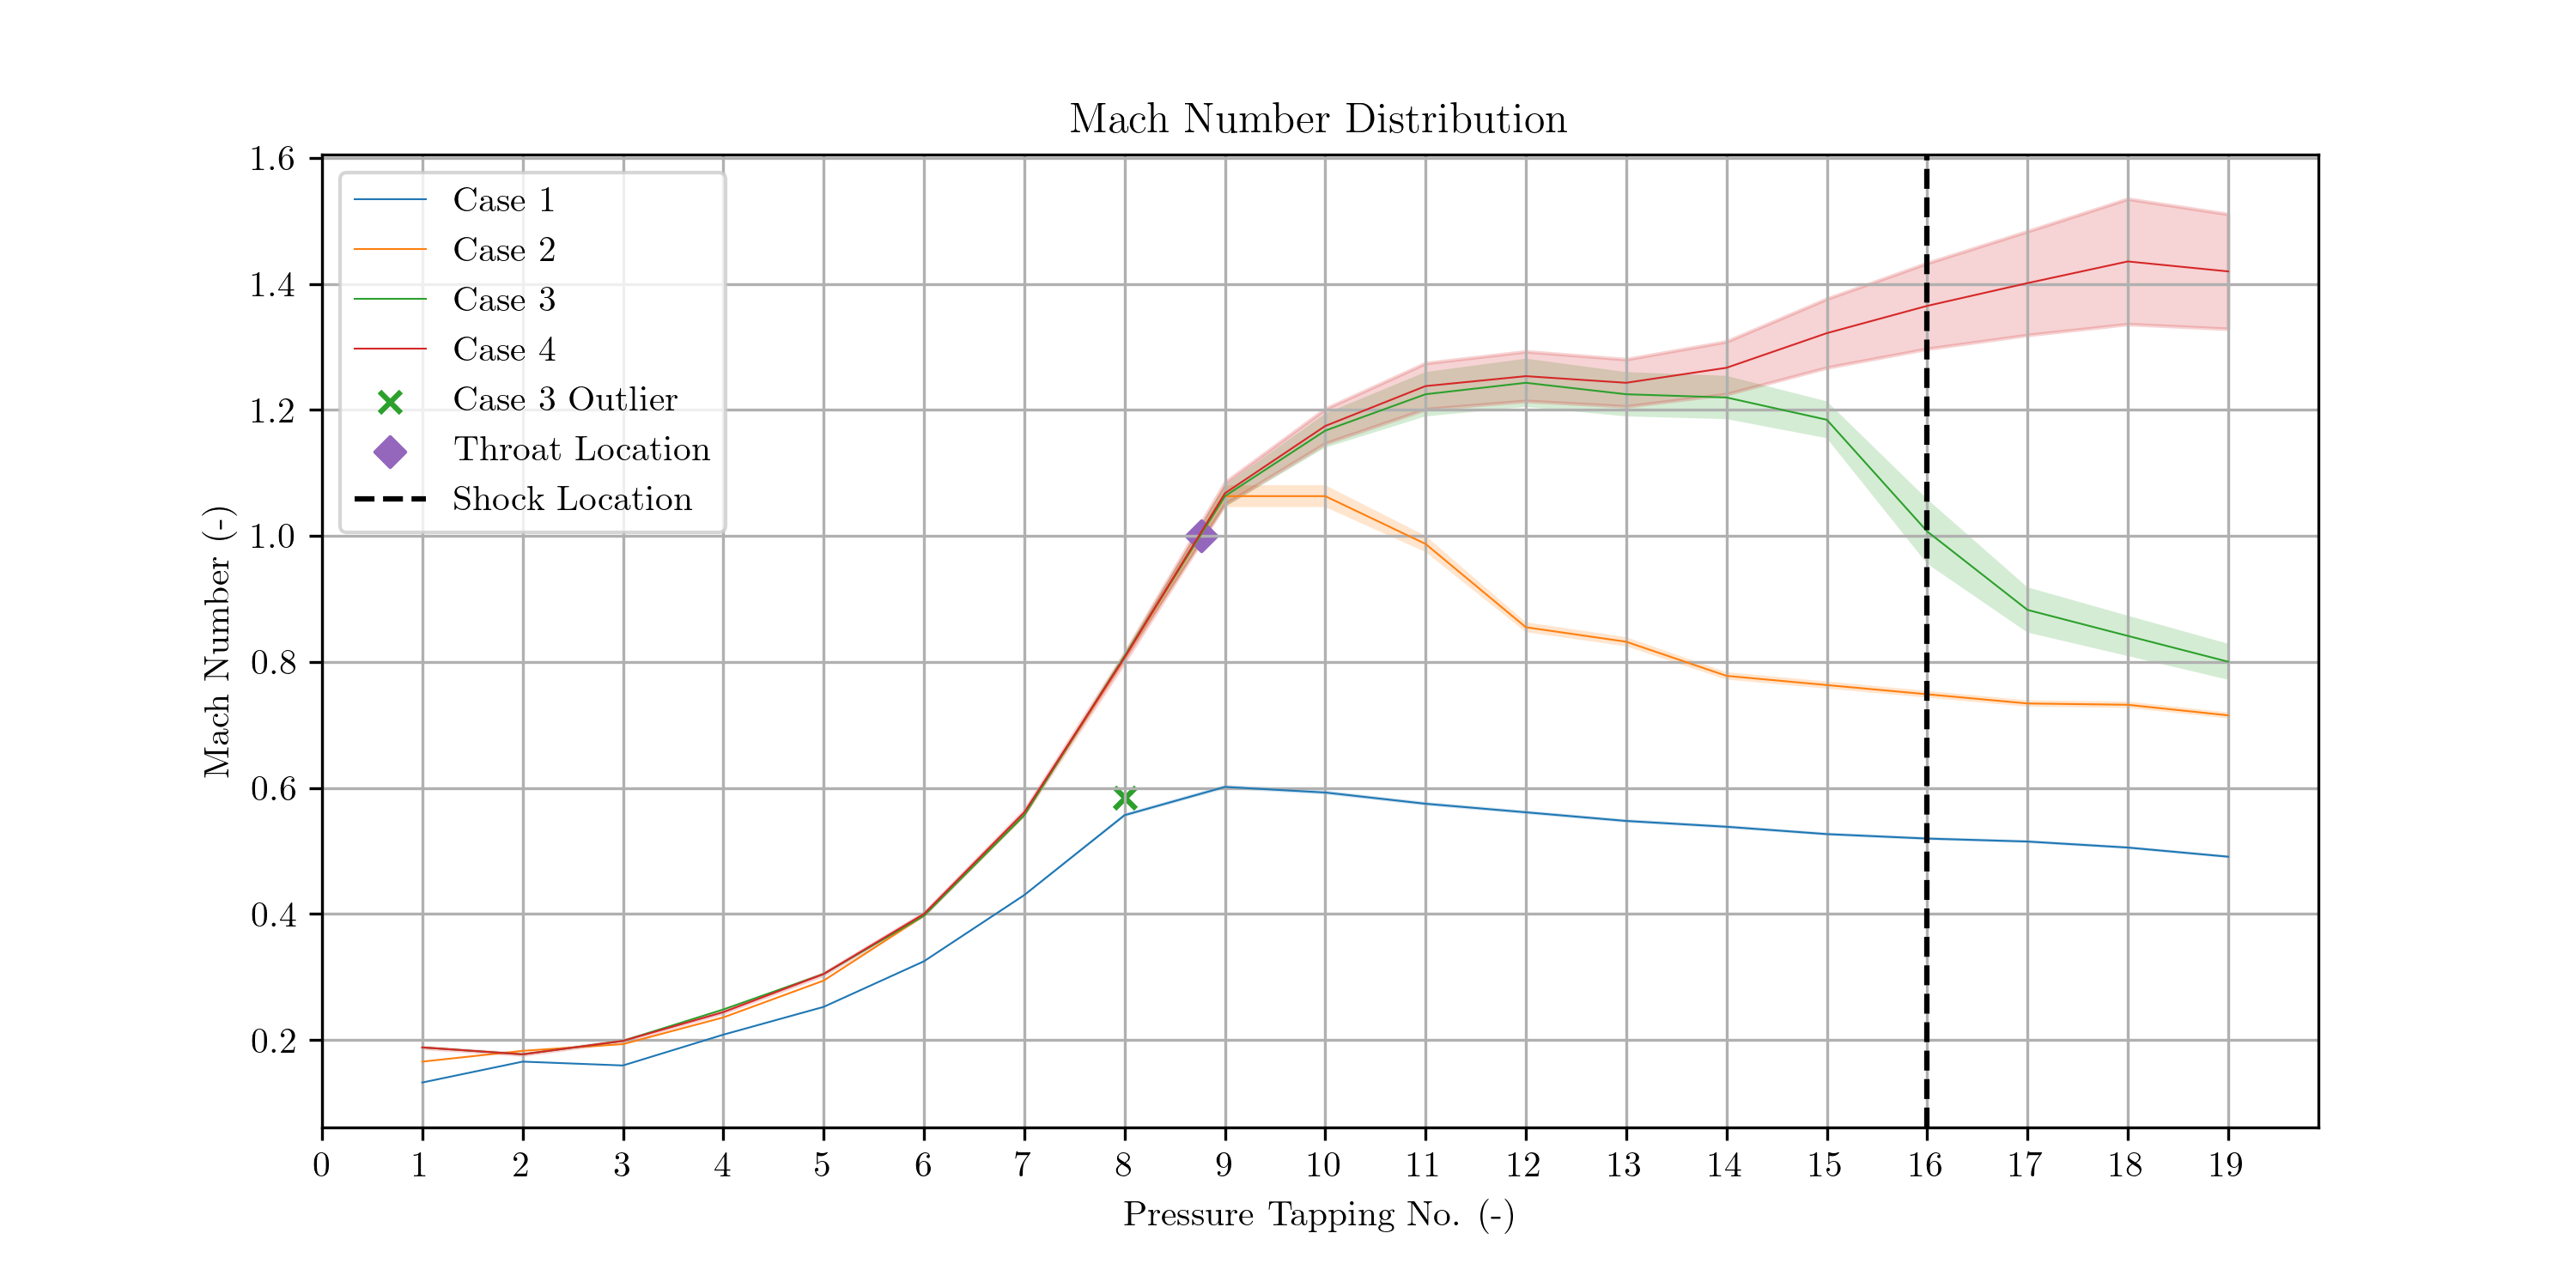
\includegraphics[width=0.98\textwidth]{../Supersonic_Nozzle/mach_number_distribution_corrected.png}
    \caption{Static pressure ratio distribution along the nozzle.}
    \label{fig:mach_distribution}
\end{figure}

\begin{figure}[H]
    \centering
    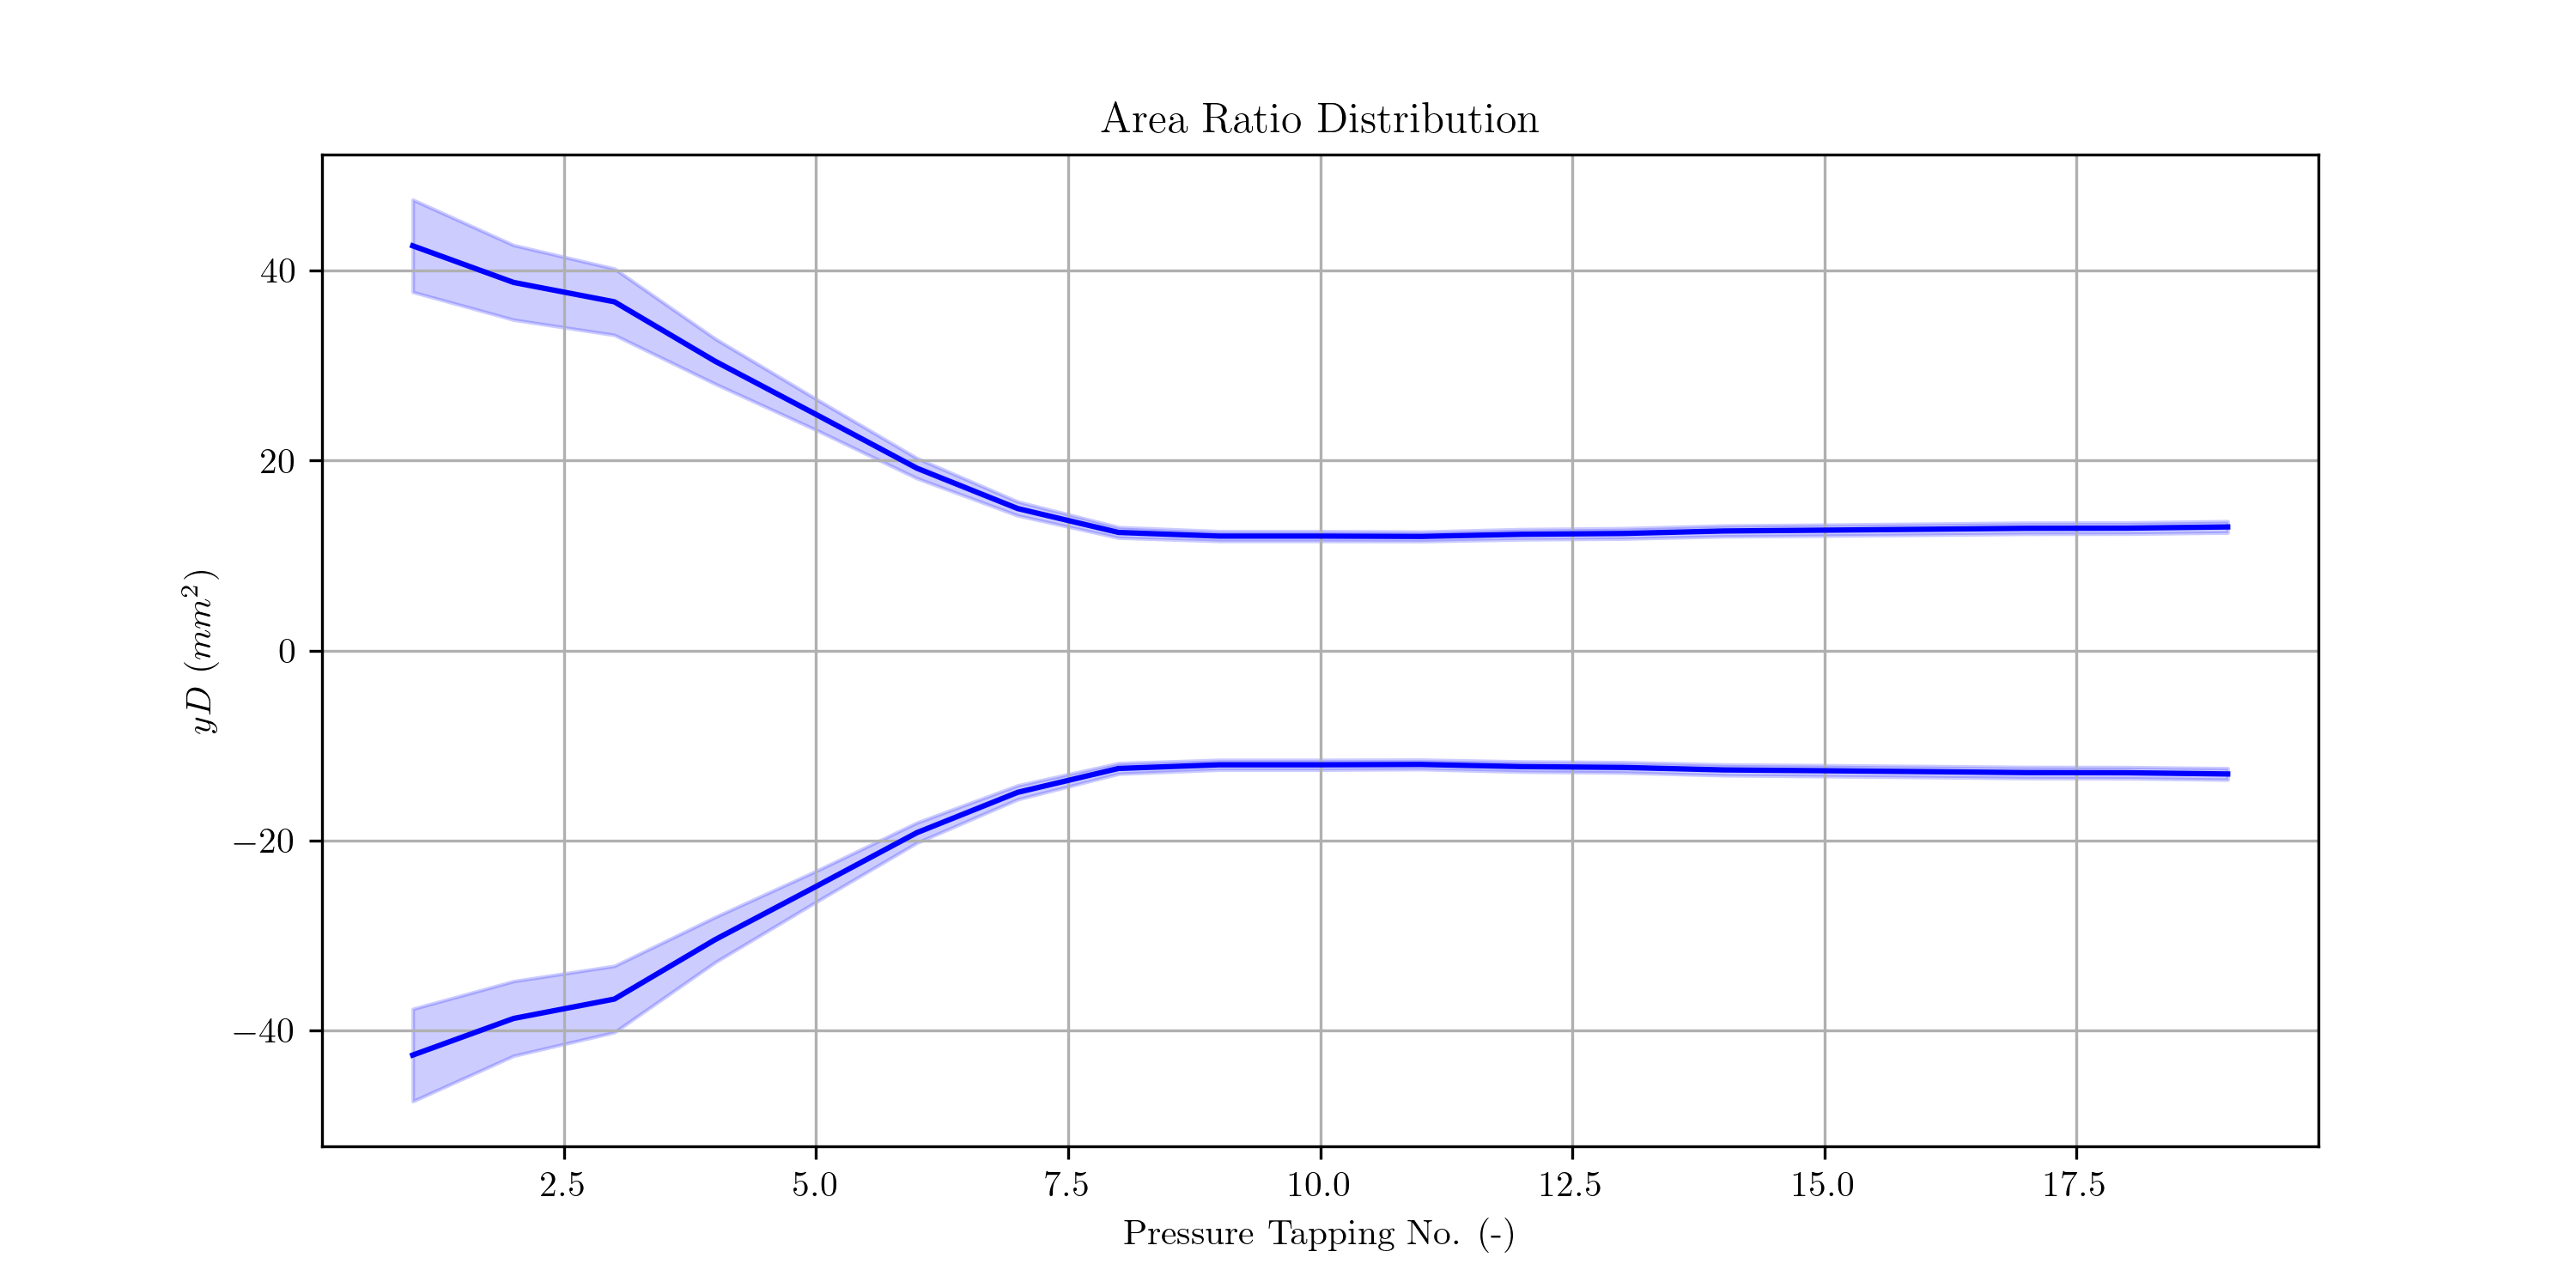
\includegraphics[width=0.98\textwidth]{../Supersonic_Nozzle/area_ratio_distribution.png}
    \caption{Reconstructed nozzle profile from throat area ratio for Case 2.}
    \label{fig:area_distribution}
\end{figure}

\begin{figure}[H]
    \centering
    \begin{subfigure}[t]{0.48\textwidth}
        \centering
        \includegraphics[width=1\textwidth]{../Supersonic_Nozzle/shadowgraph_annotations/slide1.PNG}
        \caption{Shock wave in working section before sensors}
        \label{fig:figure6}
    \end{subfigure}
    ~
    \begin{subfigure}[t]{0.48\textwidth}
        \centering
        \includegraphics[width=1\textwidth]{../Supersonic_Nozzle/shadowgraph_annotations/slide2.PNG}
        \caption{Working state and bow shock of pitot probe}
        \label{fig:figure7}
    \end{subfigure}
    \caption{Schlieren images of the supersonic wind tunnel}
\end{figure}

\begin{figure}[H]
    \centering
    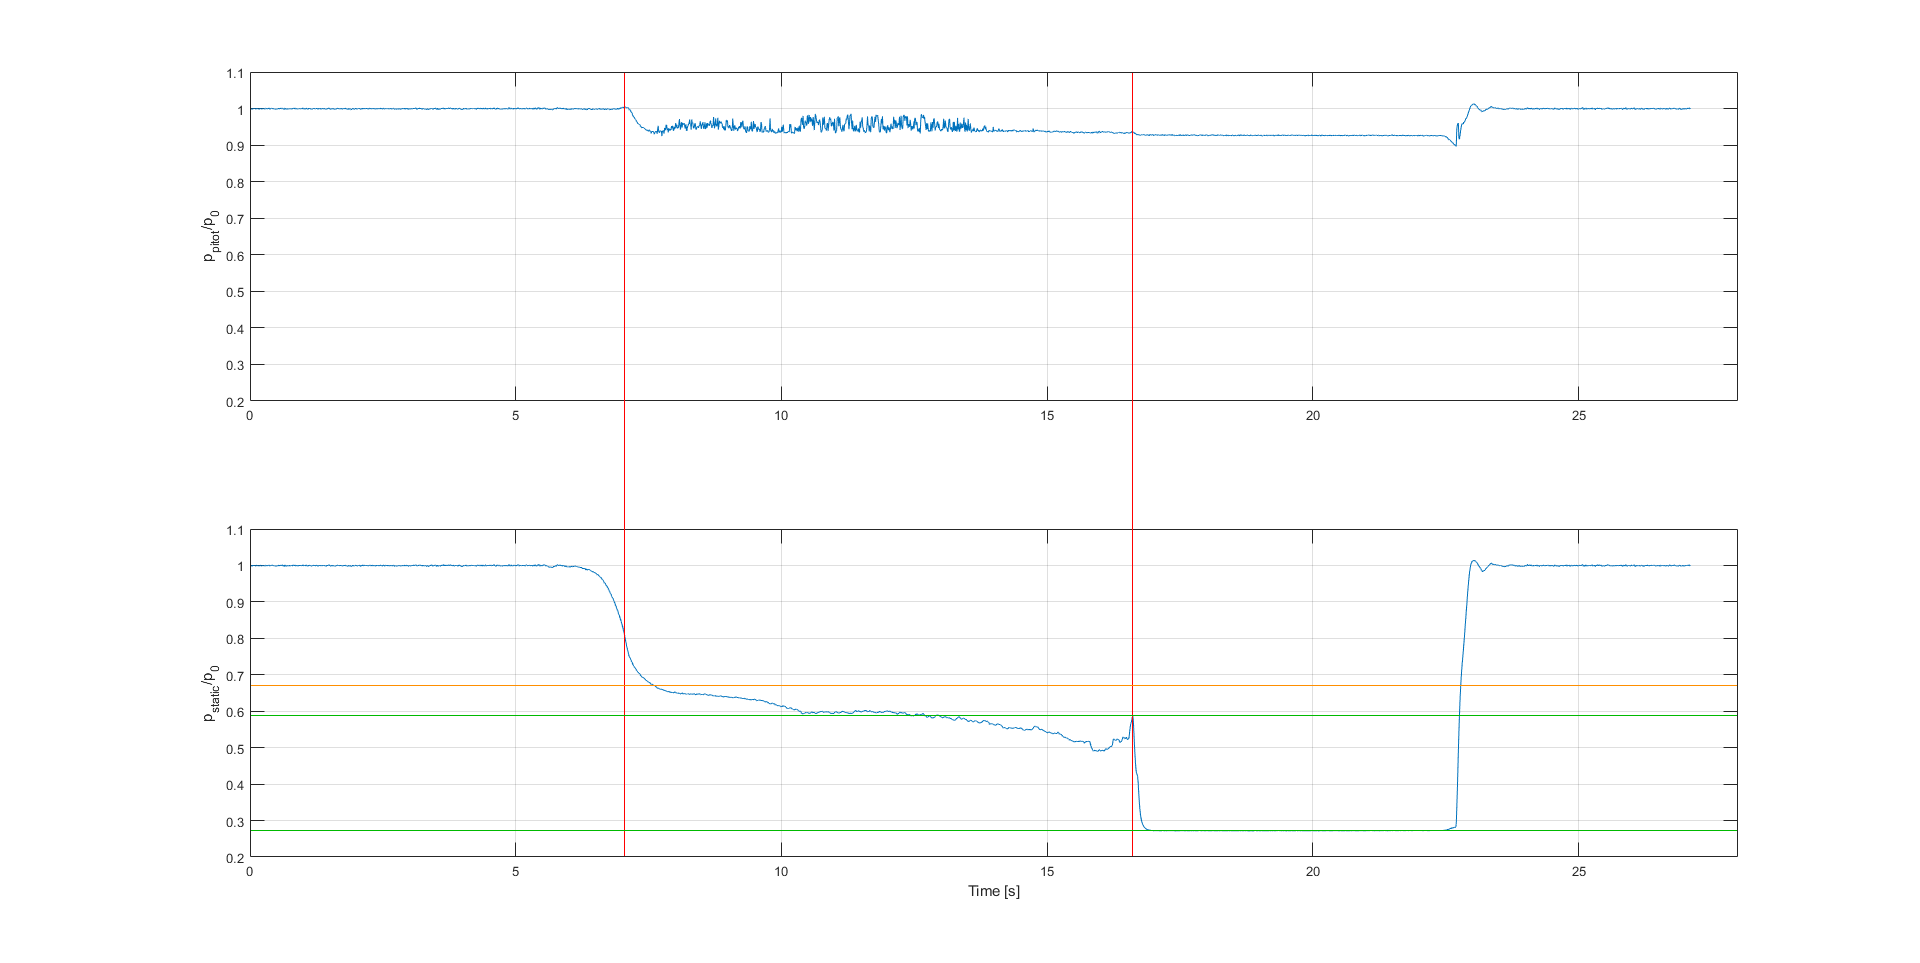
\includegraphics[width=1\textwidth]{../Supersonic_Nozzle/tunnel_pressures_annotated.png}
    \caption{Annotated readings of the pressure sensors over time during the experiment. Top graph shows the stagnation pressure ratio, and the bottom graph shows the static pressure ratio.}
    \label{fig:figure8}
\end{figure}

\newpage

\section{Discussion}

\subsection{Part 1}

Experimental results of flow behaviour for cases 1, 2 and 4 agree nicely with theory predicted for convergent and divergent sections of the nozzle discussed in theory section.
However, case 3 shows a deceleration of supersonic flow in the divergent section of the nozzle, which is thought to be due to the formation of a normal shock wave.
This was also considered in the theoretical analysis and so drop in stagnation pressure ratio is corrected for in the results.
The graphs produced ignore an outlier in the reading at tapping 8 for case 3, which is thought to be due to an error in the measurement.
The uncertainty in pressure ratio is difficult to be seen, except for after the shock in case 3, where there is additional uncertainty due to the correction for the stagnation pressure drop across the shock.

From theory of 1D normal shocks, it would be expected to see a sudden drop for case 3, indicated by the black band on the pressure graph in figure \ref{fig:pressure_distribution}
This lack of sharp jump in pressure is thought to be due to a smearing effect of the pressure at the wall, where the tappings are.
In figure \ref{fig:SBLI_pressure_smearing} the pressure distribution at the wall is shown to be smeared out by compression waves in the boundary layer.
The shock position is estimated to be at the point of Mach 1, which is an average of the Mach number before and after the shock.
This taken to be at position 16 and is indicated by the black dotted line on figure \ref{fig:pressure_distribution}.
To overcome this smearing effect, the pressure before the shock is taken to be that of Case 4 at the shock location.
From this the strength of the shock and expected pressure jump across the shock can be calculated, which is shown in figure \ref{fig:pressure_distribution}.
The calculated pressure behind the shock closely aligns with the pressure for limiting Choked Case 2, as expected.

% For run 3 of Part 1, determine the strength of the shock in the nozzle from its assumed location.
% Indicate the expected (inviscid) pressure jump across the shock on your graph.

% Using your measurement of mass flow in Part 1, calculate the cross-sectional areas of the throat and at the nozzle exit for each run.
% In the case of Run 3 you need to first determine the expected stagnation pressure drop through the shock wave before calculating the nozzle exit area. 

The graph of Mach number distribution shows significant uncertainty in the supersonic region of the nozzle.
This is due to the increased relative uncertainty of the small pressure ratios, which is propagated through the Mach number equation.
The actual cross-sectional area at the throat of the nozzle is approximately 24 mm$^2$.
However, all values calculated in table \ref{tab:1} for throat area are below this value.
The Mach numbers at the tapping closest to the throat being slightly above 1.0 for cases 2,3 and 4.
This means that the error in the calculated throat area is likely due to the rounding of throat tapping number.
However, for Case 2 the Mach number should still not be above 1.0 as it should only be on the limit of choking.
The next two pressure tappings after the throat for case 2 show that the flow is supersonic which suggests the flow passes through a weak normal shock and becomes subsonic again.
This can't be said with any confidence however, as for a weak shock as the pressure jump is both small and smeared.

Table \ref{tab:1} shows relative uncertainties of the order of 10\% in nozzle exit area for each case.
This is due to the propergated uncertainty from many calculations to find the nozzle exit area.
There is also an additional uncertainty in the location of the shock wave, which is not included in the uncertainty analysis.

Figures \ref{fig:area_distribution} and \ref{fig:actual_nozzle} show the reconstructed nozzle profile for case 2 and the actual nozzle profile respectively.
The reconstructed nozzle profile can be seen to resemble the actual nozzle profile quite well, however the exact distances between tappings may not be equal.

% You should then attempt to explain any differences you may find between the results of the different runs (note that the actual cross-sectional area at the throat of the nozzle is approximately 24 mm2).

\subsection{Part 2}

Figure \ref{fig:figure6} shows the shock wave in the working section of the supersonic wind tunnel before the pressure sensors.
It can be observed that behind there is a dark band with a light band on the right hand side.
This confirms the expected positive density gradient in the x direction.
It can also be observed that the bands of the normal shock are the widest and most distinct, indicating that this is the largest density gradient, and the strongest shock.
At the boundary layers at the top and bottom of the tunnel, the flow appears to travel through two shockwaves.
After the first shockwave the flow near the boundary layer is subsonic, but then must be accelerated again to supersonic speeds before the second, weaker shock.

Figure \ref{fig:figure8} shows the annotated readings of the pressure sensors over time during the experiment.
The green and red dots indicate the time at which the tunnel was switched on and off respectively.
It can be observed that before the first vertical red line, the static pressure decreases which corresponds to the subsonic flow accelerating.
At the first red line the stagnation pressure falls as the normal shock wave is formed upstream of the sensors by the, now supersonic, flow downstream of the throat.
The stagnation pressure readings then fluctuate as the shock wave moves further downstream due to complex shock boundary layer interactions.
The static pressure ratio slowly decreases over the next several seconds, indicating an acceleration in the flow, before quickly increasing again.
This may be due to the boundary layer growing and then shrinking rapidly, acting similarly to a convergent divergent nozzle, as the shock wave moves closer to the sensors.
The second vertical red line shows where the shock wave passes the sensors and static pressure drops significantly.

After the shock has passed, the bottom green line shows a static pressure ratio of around $p/p_0 = 0.275$. This corresponds to a Mach number of 1.49, which is very close to the set operating point of Mach 1.5.
From the databook, at Mach 1.5 the pressure ratio across the shock should be $p_s/p = 2.4583$.
Multiplying this by the measured static pressure ratio after the shock passes, gives us the theoetical static pressure ratio before the shock passed, which is $p_s/p_0 = 0.275 \times 2.4583 = 0.676$, and is shown by the orange horizontal line.
The actual pressure ratio behind the shock, given by the pressure at the time before the shock passes the sensors, is shown by the top green line at $p_s/p_0 = 0.59$.
This shows that the actual pressure drop across the shock is less than the theoretical value for Mach 1.5.
It seems that the flow downstream of the shock is at a higher Mach number than expected due to the boundary layer effects.

The pitot probe should show an increase in stagnation pressure after the shock wave passes, however it can be observed that this remains nearly unchanged.
The expected stagnation pressure ratio downstream of the shock can be calculated from Equation 8 for Mach 1.5 and is found to be 0.9298. This very close to the value seen, however after the shock passes the stagnation pressure ratio should increase back to 1.0.
It can be observed from figure \ref{fig:figure7} that a bow shock forms in front of the pitot probe and so the shock effectively never passes the probe, which explains why the stagnant pressure ratio does not increase back up to 1.0.
This is why the ratio of Pitot pressure to inlet stagnation pressure is almost independent of shock position.

\subsection{Comparison of Part 1 and Part 2}
% Compare the two experiments. Are there any findings that can be related from one experiment to the other?
% What have you learned about the interaction of a shock wave with a boundary layer?

In both experiments, the shock wave is observed to be the strongest in the free stream, away from the boundary layer.
This is because the flow is not slowed down by viscous effects and so can undergo a shock at a higher Mach number.
Unsteady shock boundary layer interactions are also observed in both experiments.
In Part 1, the wall pressure distribution near the shock is smeared by compression waves in the boundary layer.
In Part 2, the stagnant pressure fluctuates as the shock wave moves closer to the sensors, which indicate unsteady shock boundary layer interactions.


\section{Conclusion}
% Comment on the validity of one-dimensional theory in nozzle flows. When can it be expected to provide what quality of predictions?
% What are the effects of viscosity in both experiments? Which experiment is more severely affected and why?

Experimental results of flow behaviour for cases 1, 2 and 4 agree nicely with one-dimensional theory discussed.
The pressure distribution for Case 3 shows a deceleration of supersonic flow due to a normal shock.
However, theory of one dimensional normal shocks predicts a sharp jump in pressure, which is not observed.
This was later determined to be due to a smearing effect of the viscous boundary layer at wall pressure measurements near to the shock \cite{babinsky_delery:2011}.
This effect severely affected pressure readings in Part 1, however this did not effect part 2 where the pressure sensors were located in the free-stream, away from the boundary layer.
Choking was observed in cases 2, 3 and 4 by identical mass flow rates and the location of the throat was found to be between tappings 8 and 9.
Calculated values for throat area and exit area from mass flow rate show a large variation, which is due to the propagated uncertainty from many calculations.
The centralised area to throat area ratio, plotted for case (\ref{fig:area_distribution}), resembles the actual nozzle profile (\ref{fig:actual_nozzle}).
On startup of the supersonic wind tunnel, a normal shock wave is observed to move downstream through the working section on the shadowgraph.
The shock wave is observed to be the strongest in the free stream, away from the boundary layer.
The pressure drop accross the shock appears smaller than the theoretical value for Mach 1.5, which suggests the flow downstream of the shock is higher than expected.
This is thought to be due to the boundary layer acting as a converging nozzle and accelerating the flow downstream of the shock.


%%%%%%%%%%%%%%%%%%%%%%%%%%%%%%%%%%%%%%%%%%%%%%%%%%%%%%%%%%%%%%%%%%%%%%%%%%%%%%%%%%%%%%%%%%%%

\iftrue

\newpage
\section{Appendix}

\subsection{Schlieren visualisation technique}

\begin{figure}[H]
    \centering
    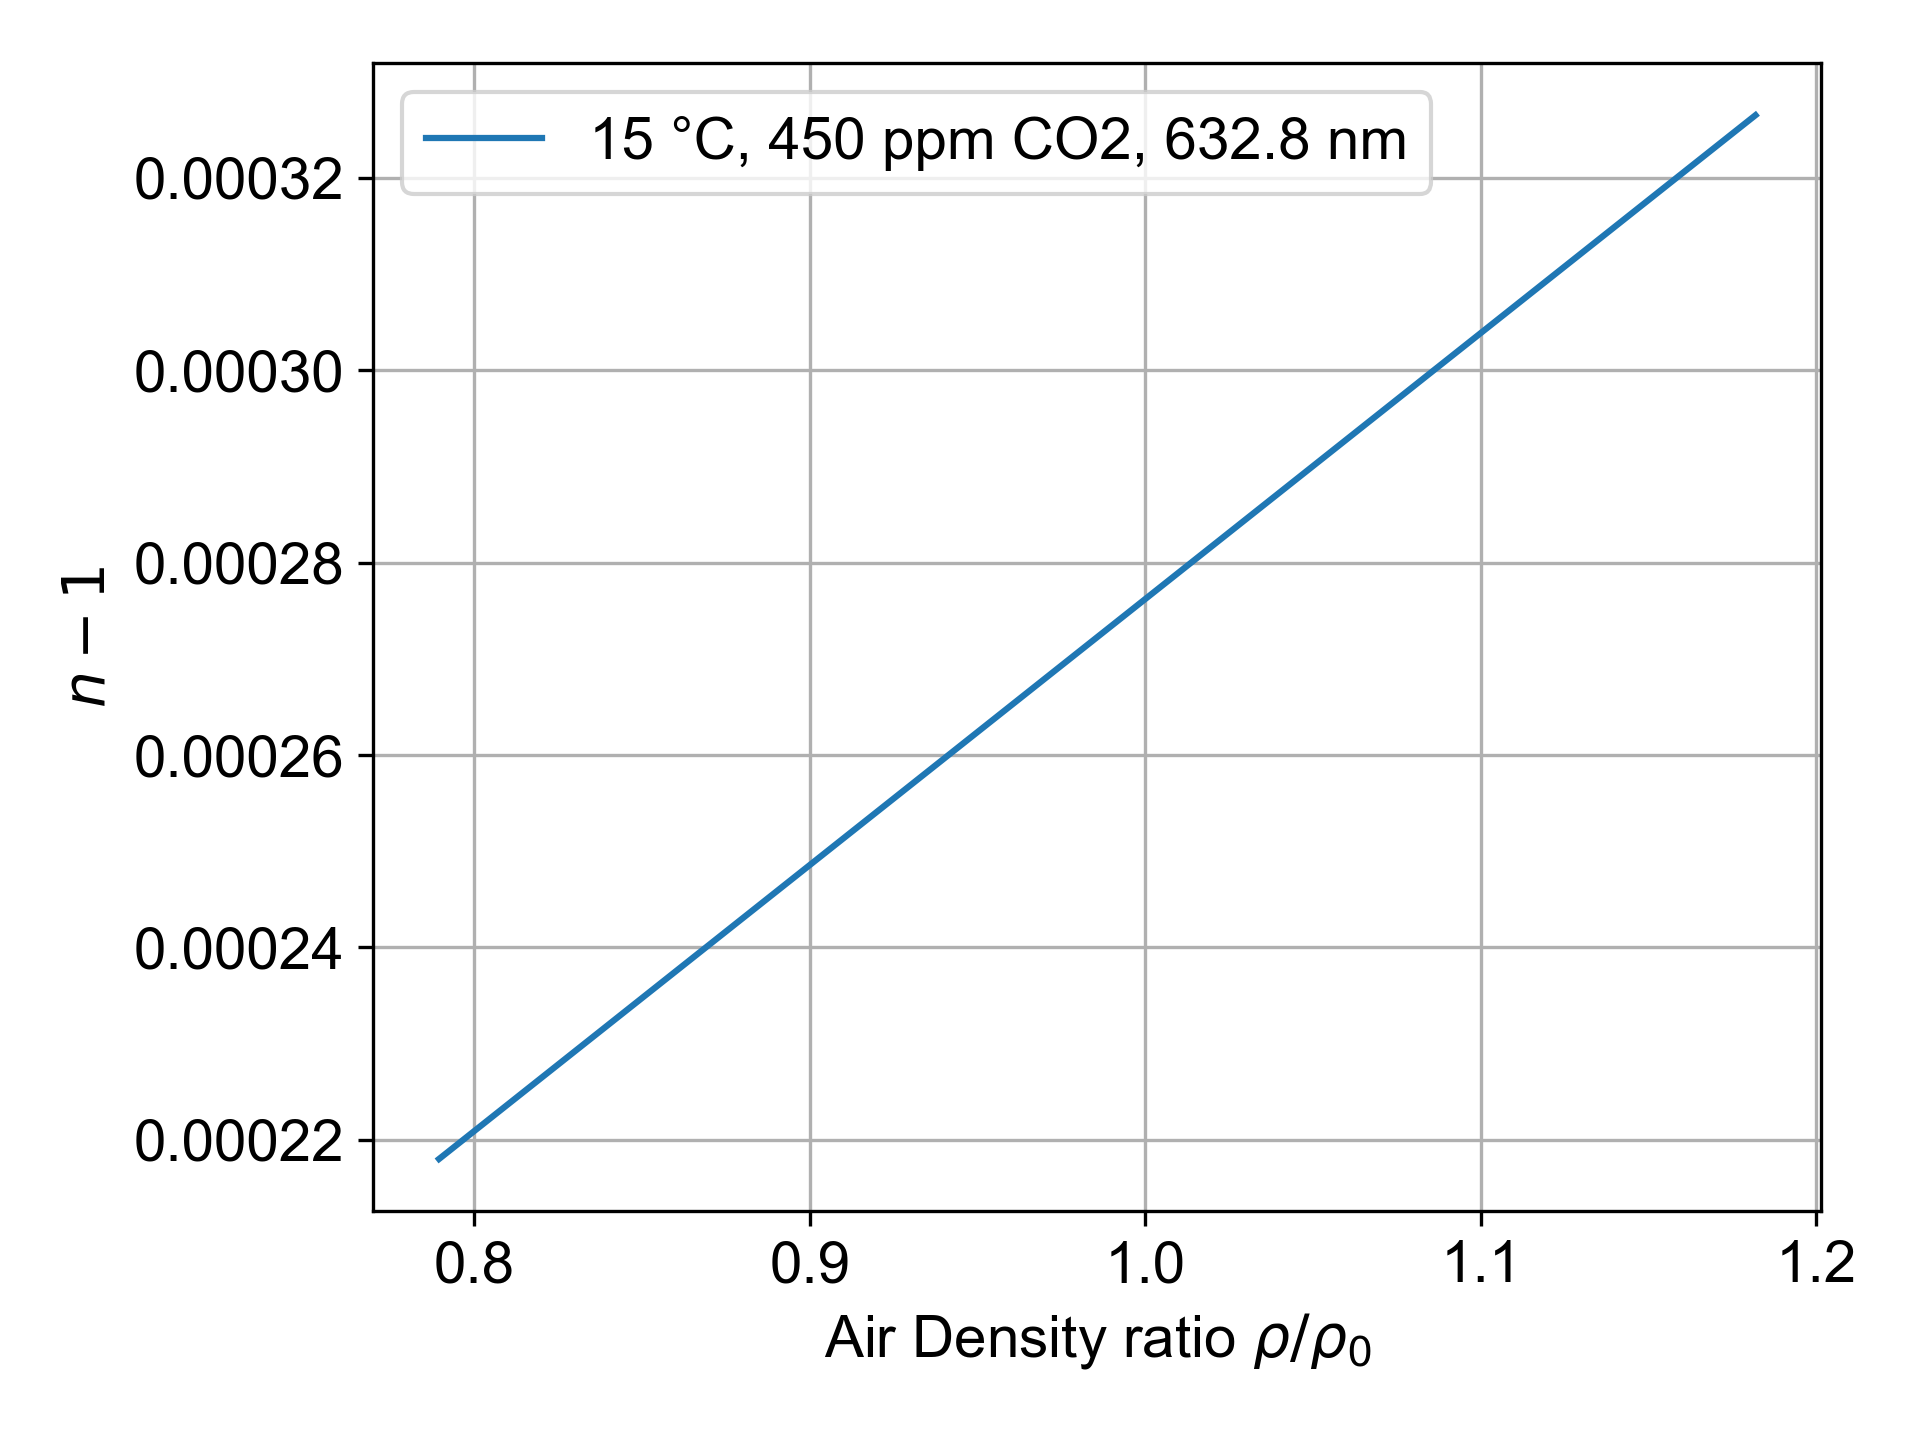
\includegraphics[width=0.6\textwidth]{dry_air_15_rho_vs_n.png}
    \caption{Refractive index $n-1$ against density ratio $\rho/\rho_0$ for relative humidity $\phi = 50\%$, 450 ppm $ \text{CO}_2 $, wavelength $\lambda = 632.8$ nm. Figure produced from modified code \cite{refractiveindex_info} using equations by Ciddor, 1996 \cite{Ciddor:96}.}
    \label{fig:refractive_index_vs_density}
\end{figure}

\begin{figure}[H]
    \centering
    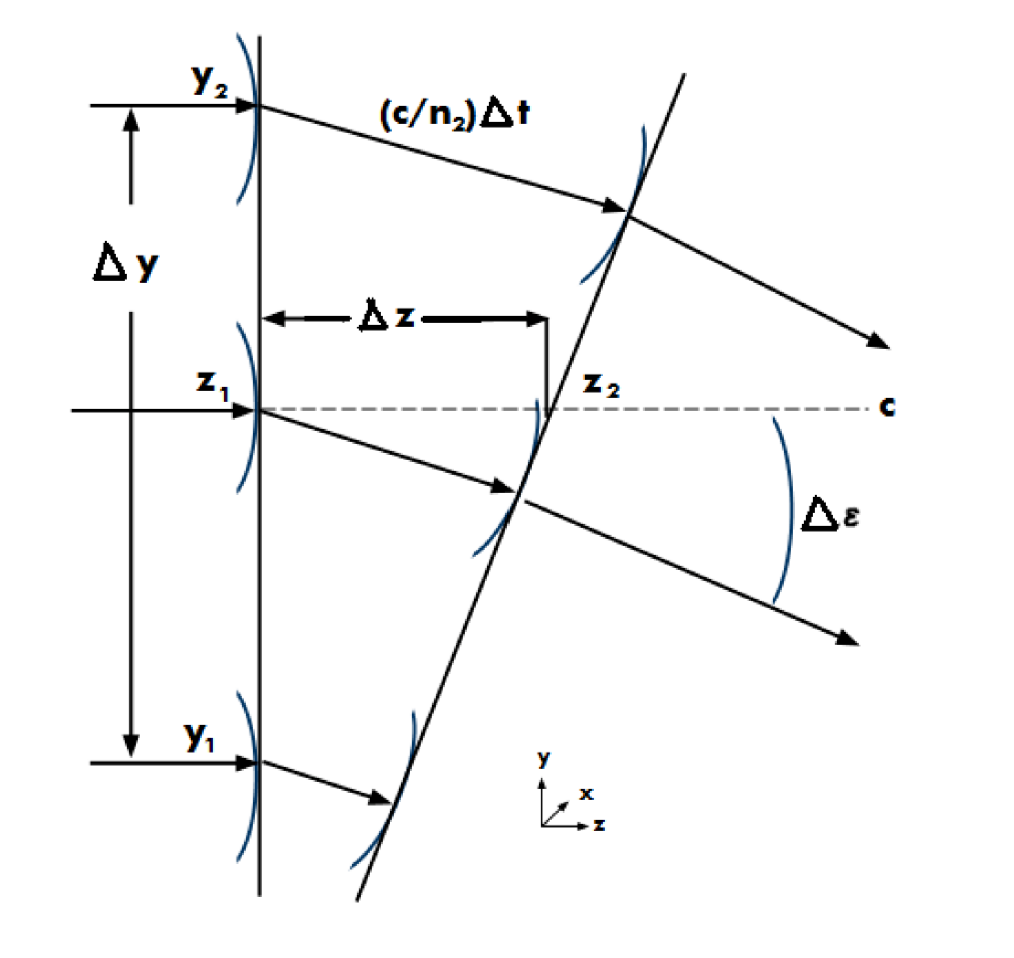
\includegraphics[width=0.5\textwidth]{Mazumdar_Amrita_shlierien_refraction.png}
    \caption{Top down view of light ray deflection by refractive indicies $n_2 < n_1$ and so gradient $\partial n/ \partial y < 0$ \cite{Mazumdar_Amrita:2013}.}
    \label{fig:refraction_diagram}
\end{figure}
Equations showing the relationship between refractive index gradients and ray deflection angles are derived by Mazumdar \cite{Mazumdar_Amrita:2013} and shown below.
\begin{equation}
    \epsilon_y = \frac{1}{n}\int \frac{\partial n}{\partial y} dz \;\;\;\;\;\; \epsilon_x = \frac{1}{n}\int \frac{\partial n}{\partial x} dz
    \label{eqn:refractive_index_gradient}
\end{equation}

\subsection{Further uncertainty analysis}

The following equations are used to calculate uncertainty in nozzle area and dimensionless mass flow rate.

\begin{equation}
    u\left( \frac{A}{A^*} \right) = u(M) \frac{d}{dM}\left( \frac{A}{A^*} \right) \;\;\;\;\;\;\;\;\;\;\;\; u\left( \frac{\dot{m}\sqrt{c_pT_0}}{p_0A} \right) = u(M) \frac{d}{dM}\left( \frac{\dot{m}\sqrt{c_pT_0}}{p_0A} \right)
\end{equation}

\begin{equation}
    \frac{d}{dM}\left( \frac{A}{A^*} \right) = \frac{2 \left(\frac{2 \left(M^{2} \left(\frac{\gamma}{2} - \frac{1}{2}\right) + 1\right)}{\gamma + 1}\right)^{\frac{\gamma + 1}{2 \gamma - 2}} \left(\frac{\gamma}{2} - \frac{1}{2}\right) \left(\gamma + 1\right)}{\left(2 \gamma - 2\right) \left(M^{2} \left(\frac{\gamma}{2} - \frac{1}{2}\right) + 1\right)} - \frac{\left(\frac{2 \left(M^{2} \left(\frac{\gamma}{2} - \frac{1}{2}\right) + 1\right)}{\gamma + 1}\right)^{\frac{\gamma + 1}{2 \gamma - 2}}}{M^{2}}
    \label{eqn:dA_dM}
\end{equation}

\begin{equation}
    \frac{d}{dM}\left( \frac{\dot{m}\sqrt{c_pT_0}}{p_0A} \right) = \frac{2 M^{2} \gamma \left(- \gamma - 1\right) \left(\frac{\gamma}{2} - \frac{1}{2}\right) \left(M^{2} \left(\frac{\gamma}{2} - \frac{1}{2}\right) + 1\right)^{\frac{- \gamma - 1}{2 \gamma - 2}}}{\sqrt{\gamma - 1} \cdot \left(2 \gamma - 2\right) \left(M^{2} \left(\frac{\gamma}{2} - \frac{1}{2}\right) + 1\right)} + \frac{\gamma \left(M^{2} \left(\frac{\gamma}{2} - \frac{1}{2}\right) + 1\right)^{\frac{- \gamma - 1}{2 \gamma - 2}}}{\sqrt{\gamma - 1}}
    \label{eqn:dmdot_dM}
\end{equation}

The following equations are used to correct for the drop in stagnation pressure across the shock wave in Case 3.

\begin{equation}
    \frac{p_{0s}}{p_0} = \left( \frac{\frac{\gamma+1}{2}M^2}{1 + \frac{\gamma-1}{2}M^2}\right) ^ \frac{\gamma}{\gamma-1} \left( \frac{2\gamma}{\gamma+1} M^2 - \frac{\gamma-1}{\gamma+1}\right) ^ \frac{1}{1 - \gamma}
\end{equation}

\begin{equation}
    u\left( \frac{p_{0s}}{p_0} \right) = u(M) \frac{d}{dM}\left( \frac{p_{0s}}{p_0} \right)
\end{equation}

\begin{equation}
    \begin{aligned}[b]
    & \frac{d}{dM}\left( \frac{p_{0s}}{p_0} \right) = - \frac{4 M \gamma \left(\frac{M^{2} \left(\frac{\gamma}{2} + \frac{1}{2}\right)}{M^{2} \left(\frac{\gamma}{2} - \frac{1}{2}\right) + 1}\right)^{\frac{\gamma}{\gamma - 1}} \left(\frac{2 M^{2} \gamma}{\gamma + 1} - \frac{\gamma - 1}{\gamma + 1}\right)^{- \frac{1}{\gamma - 1}}}{\left(\gamma - 1\right) \left(\gamma + 1\right) \left(\frac{2 M^{2} \gamma}{\gamma + 1} - \frac{\gamma - 1}{\gamma + 1}\right)} \\
    & + \frac{\gamma \left(\frac{M^{2} \left(\frac{\gamma}{2} + \frac{1}{2}\right)}{M^{2} \left(\frac{\gamma}{2} - \frac{1}{2}\right) + 1}\right)^{\frac{\gamma}{\gamma - 1}} \left(M^{2} \left(\frac{\gamma}{2} - \frac{1}{2}\right) + 1\right) \left(\frac{2 M^{2} \gamma}{\gamma + 1} - \frac{\gamma - 1}{\gamma + 1}\right)^{- \frac{1}{\gamma - 1}} \left(- \frac{2 M^{3} \left(\frac{\gamma}{2} - \frac{1}{2}\right) \left(\frac{\gamma}{2} + \frac{1}{2}\right)}{\left(M^{2} \left(\frac{\gamma}{2} - \frac{1}{2}\right) + 1\right)^{2}} + \frac{2 M \left(\frac{\gamma}{2} + \frac{1}{2}\right)}{M^{2} \left(\frac{\gamma}{2} - \frac{1}{2}\right) + 1}\right)}{M^{2} \left(\frac{\gamma}{2} + \frac{1}{2}\right) \left(\gamma - 1\right)}
    \end{aligned}
    \label{eqn:dp0sr_dm}
\end{equation}

\footnotetext{Equations for derivatives \ref{eqn:dA_dM}, \ref{eqn:dmdot_dM} and \ref{eqn:dp0sr_dm} were generated using SymPy from databook equations \cite{data_book}.}

\subsection{Additional figures}

\begin{figure}[H]
    \centering
    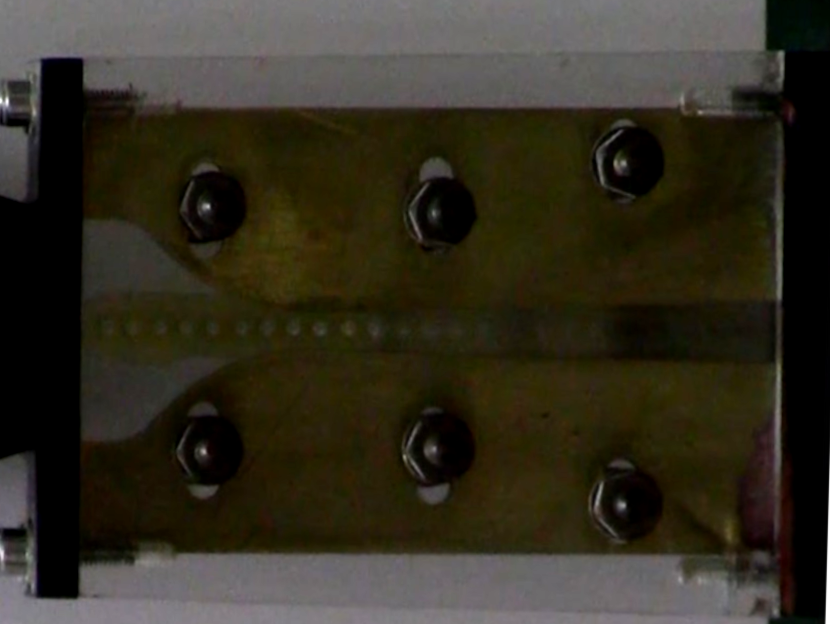
\includegraphics[width=0.7\textwidth]{actual_nozzle_profile.png}
    \caption{Transformed and colour corrected image of actual nozzle profile.}
    \label{fig:actual_nozzle}
\end{figure}

\begin{figure}[H]
    \centering
    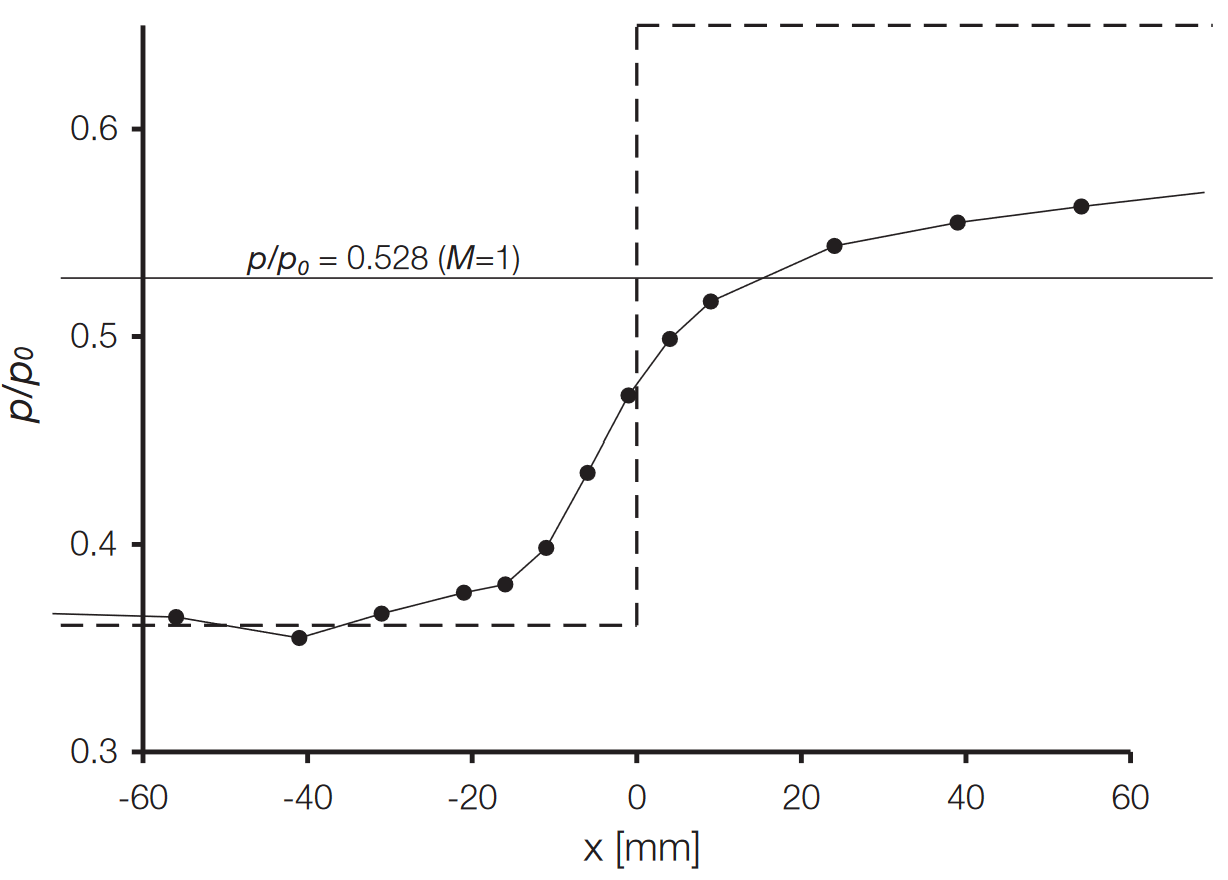
\includegraphics[width=0.6\textwidth]{SBLI_pressure_smearing.png}
    \caption{Static wall pressure distribution at the shock boundary layer interaction \cite{babinsky_delery:2011}.}
    \label{fig:SBLI_pressure_smearing}
\end{figure}

\begin{figure}[H]
    \centering
    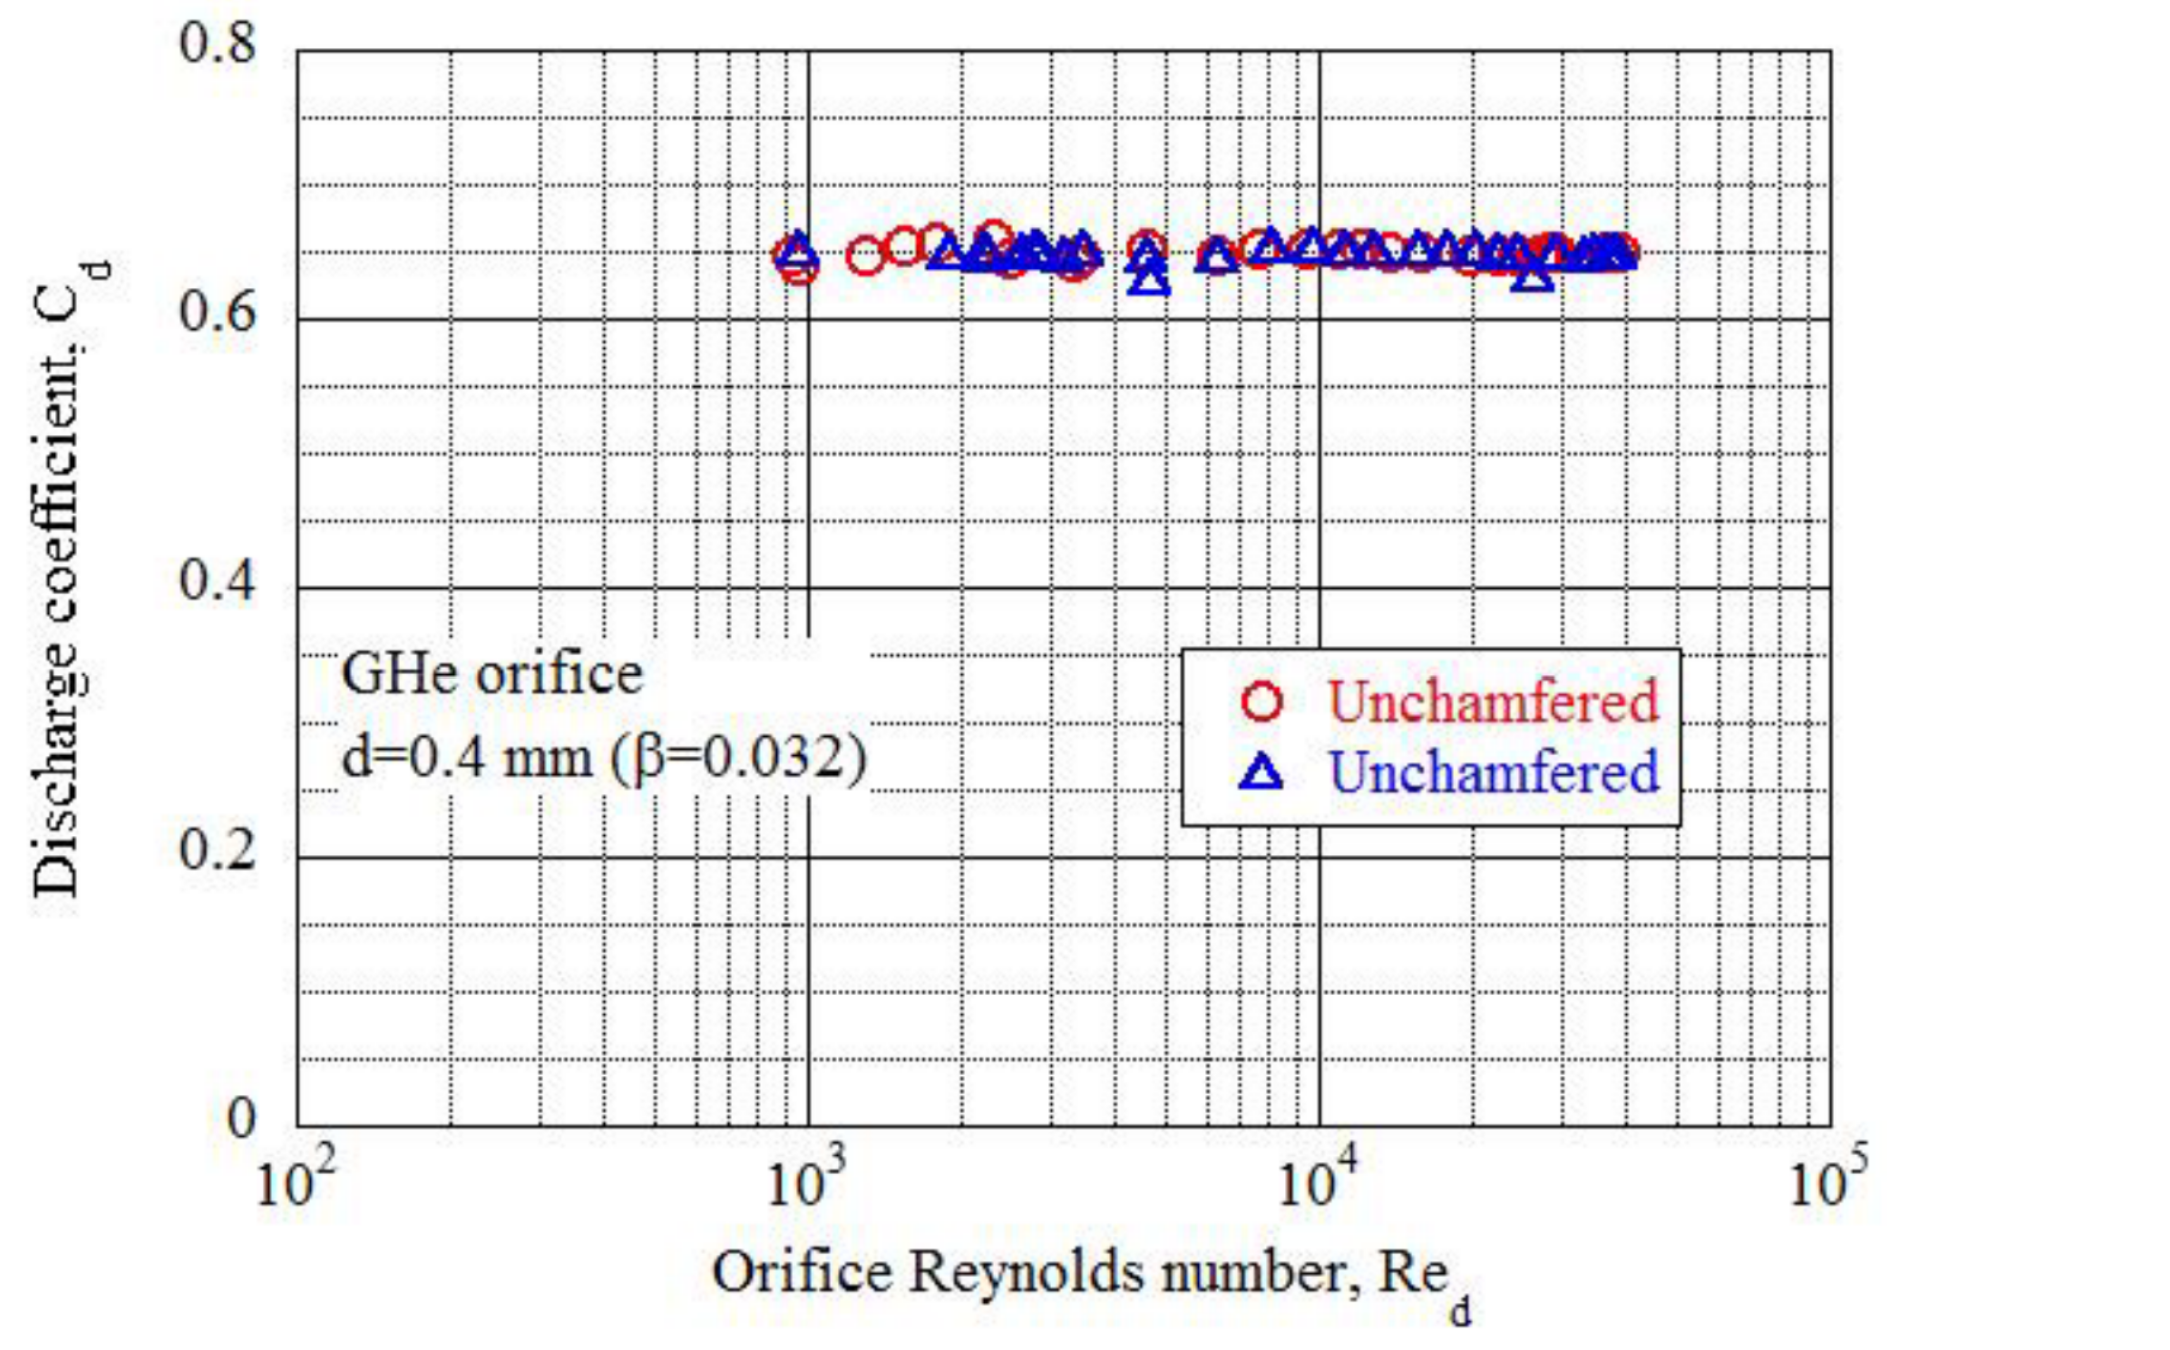
\includegraphics[width=0.8\textwidth]{Graham_K_Webster_const_Cd_Re.png}
    \caption{Constant discharge coefficient for high Reynolds numbers \cite{Graham_K_Webster:2019}.}
    \label{fig:const_Cd_Re}
\end{figure}

\fi

\bibliographystyle{plain}
\bibliography{refs}

\end{document}